\documentclass[11pt]{amsart}
\usepackage[margin=1.05in]{geometry}
\usepackage{amsmath,amssymb,amsthm,mathtools}
\usepackage{booktabs}
\usepackage{listings}
\usepackage{xcolor}
\usepackage[hidelinks]{hyperref}
\usepackage{url}
\usepackage{xurl}
\usepackage[T1]{fontenc}
\usepackage{graphicx}
\usepackage{seqsplit}
\sloppy
\allowdisplaybreaks
\graphicspath{{figures/}}

\newtheorem{theorem}{Theorem}[section]
\newtheorem{proposition}[theorem]{Proposition}
\newtheorem{lemma}[theorem]{Lemma}
\newtheorem{corollary}[theorem]{Corollary}
\theoremstyle{definition}
\newtheorem{definition}[theorem]{Definition}
\theoremstyle{remark}
\newtheorem{remark}[theorem]{Remark}

\lstset{basicstyle=\ttfamily\footnotesize,columns=fullflexible,keepspaces=true,
  frame=single,framerule=0.3pt,xleftmargin=0.5em,xrightmargin=0.5em,
  breaklines=true,breakatwhitespace=false,postbreak=\mbox{\textcolor{gray}{$\hookrightarrow$}\space},
  escapeinside={(*}{*)}}

\newcommand{\Lin}{\mathcal{L}}
\newcommand{\Prob}{\mathbf{P}}
\newcommand{\Wdag}{\mathcal{W}_2^{\dagger}}
\newcommand{\deltadag}{\delta_2^{\dagger}}

\newcommand{\pin}{1ff4fad}
\newcommand{\mk}[1]{\mathtt{#1}}

\title[Small balance constants for width-two posets]{Small Balance Constants for Width-Two Posets}

\author[Neil Xu]{Neil Xu\\[2pt]{\normalfont\small\texttt{\lowercase{neard.ws@gmail.com}}}}

\date{October 2026}

\begin{document}

\begin{abstract}
For a finite poset $P$ that is not a chain, the balance constant $\delta(P)$ is the largest value of $\min\{\Prob(x<y),\Prob(y<x)\}$ over pairs of elements, for a uniformly random linear extension. Let $\Wdag$ be the class of finite width-two posets that are not ordinal sums of singletons and three-element equality cases, and $\deltadag=\inf_{P\in\Wdag}\delta(P)$. We construct an explicit indecomposable family $(P_m)_{m\ge0}\subset\Wdag$ of broken-rung ladders on $108+20m$ elements, with a period-$5$ core and new end caps, for which
\[
\delta(P_m)=\frac{N_m}{E_m}\longrightarrow \alpha=\frac{115713181619-36\sqrt{6697}}{331705168868}\approx 0.348843459593420.
\]
Changing the caps gives two further families with limits $\gamma<\beta<\alpha$, and a finite $248$-element example $P^\dagger$ with $\delta(P^\dagger)<\gamma$. Every finite member of the three families, their three limits, and $P^\dagger$ lie strictly below the smallest previously published exact value known to us, $c_P\approx0.3488434604$ (Peczarski's $50$-element ladder), hence below Sah's constant $\sigma_{\mathrm S}$. The identity $\delta(P_m)=N_m/E_m$ for every $m$, starting from the generating relations of $P_m$, and the limit $\alpha$ are formalized in Lean~4 with Mathlib (standard axioms only). The families $\beta,\gamma$ are proved by exact rational-arithmetic certificates that are not formalized. The results are upper bounds on $\deltadag$; they say nothing new about the $1/3$--$2/3$ conjecture itself.
\end{abstract}

\maketitle

\section{Introduction}

Let $P$ be a finite poset and let $\Lin(P)$ be its set of linear extensions. For $x,y\in P$, write $\Prob(x<y)$ for the fraction of $L\in\Lin(P)$ in which $x$ precedes $y$. The \emph{balance constant} of $P$ is
\[
\delta(P)=\max_{x\neq y}\ \min\{\Prob(x<y),\Prob(y<x)\}.
\]
Comparable pairs contribute $0$, so the maximum may equivalently be taken over incomparable pairs. Write
\[
\delta^*=\inf\{\delta(P): P \text{ finite, not a chain}\}.
\]

\begin{quote}
\textbf{$1/3$--$2/3$ conjecture} (Kislitsyn~\cite{Kis68}, Fredman~\cite{Fre76}, Linial~\cite{Lin84}). If $P$ is a finite poset that is not a chain, then $\delta(P)\ge 1/3$.
\end{quote}

The bound $1/3$ is sharp: it is attained by the three-element poset consisting of a two-element chain and an isolated point. In particular $\delta^*\le 1/3$, with or without the conjecture. A Lean statement of the conjecture is in the formal-conjectures repository~\cite{FC}.

\subsection*{Lower bounds}
Kahn and Saks~\cite{KS84} proved $\delta(P)\ge 3/11$. Brightwell, Felsner and Trotter~\cite{BFT95} improved this to $(5-\sqrt5)/10\approx0.2764$. Their argument also applies to infinite posets $P$ that are \emph{thin} (each element is incomparable with at most $k$ others, for a fixed $k$) and \emph{locally finite} (each set $\{z:x<z<y\}$ is finite); such $P$ is countable. Take finite sets $X_1\subseteq X_2\subseteq\cdots$ with union $P$, each convex ($u,v\in X_n$ and $u<w<v$ imply $w\in X_n$). Then $\Prob(x<y)$ is defined as the limit of $\Prob(x<y)$ under the uniform distribution on the linear extensions of $P|_{X_n}$. Brightwell~\cite{Bri88} showed that this limit exists and does not depend on the sequence; see~\cite[Section~7]{BFT95}, where the bound is also extended to thin posets that are not locally finite. In this sense the poset on $\{x_i:i\in\mathbb{Z}\}$ with $x_i<x_j$ iff $j>i+1$ attains $(5-\sqrt5)/10$, so the bound is best possible for thin posets~\cite[Theorem~1.4]{BFT95}. Recently Aires, Chan, Pak and Panova~\cite{ACPP26} proved $\delta(P)\ge(5-\sqrt5)/10+\varepsilon$ for an explicit but very small $\varepsilon>0$. The conjecture is known for many special classes, for example width two~\cite{Lin84}, height two~\cite{TGF92}, $5$-thin~\cite{BW92} and $6$-thin~\cite{Pec08} posets, and all posets with at most $14$ elements~\cite{Gup26}. See~\cite{Bri99,ACPP26} for fuller lists.

\subsection*{The restricted width-two problem}
For posets $Q$ and $R$, the \emph{ordinal (linear) sum} $Q\oplus R$, called the direct sum in~\cite{Sah21}, is the disjoint union of $Q$ and $R$, with their own orders, in which every element of $Q$ is below every element of $R$. Among width-two posets, $\delta(P)=1/3$ holds only for ordinal sums built from singletons and the three-element example above (Aigner~\cite{Aig85}). The interesting extremal question is therefore the gap above $1/3$ after these equality cases are excluded. Following Sah~\cite{Sah21}, put
\[
\begin{aligned}
\Wdag=\bigl\{P:\ &P\text{ is finite of width two, and $P$ is not an ordinal}\\
&\text{sum of singletons and three-element equality cases}\bigr\},
\end{aligned}
\qquad
\deltadag=\inf_{P\in\Wdag}\delta(P).
\]
Sah proved $\delta(P)\ge(-3+5\sqrt{17})/52\approx0.33876$ for every $P\in\Wdag$. The class $\Wdag$ also contains decomposable posets: if $P\in\Wdag$ and $C_k$ is a $k$-element chain, then $P\oplus C_k\in\Wdag$ and $\delta(P\oplus C_k)=\delta(P)$, because the elements of $C_k$ are comparable to everything and the linear extensions of $P\oplus C_k$ are those of $P$ followed by $C_k$. Our constructions are indecomposable (Lemma~\ref{lem:wdag}); this is an additional goal, not part of the definition of $\Wdag$.

\subsection*{Previous upper constructions}
Chen~\cite{Chen18} gave a family of broken-rung ladders with limit $(93-\sqrt{6697})/32\approx0.3488999$. Peczarski~\cite{Pec19} searched ladders with broken rungs by computer; his $50$-element ladder $L_{50,1,5,8,9,12,13,17,20,21,25,26,29,33,34,37,38,41,45}$ has
\[
c_P=\frac{39148472052}{112223608848}=\frac{1087457557}{3117322468}\approx0.348843460426
\]
\cite[Table~2]{Pec19}; Chen's published paper also records this value~\cite[\S1.4]{Chen18}, and we recomputed it. Sah~\cite{Sah21} constructed posets $T_n$ with $\delta(T_n)\to\sigma_{\mathrm S}:=(5864893+27\sqrt{57})/16812976\approx0.348843467422$ (denoted $\beta$ by Sah) and conjectured that $\delta(P)\ge\sigma_{\mathrm S}$ for every finite $P\in\Wdag$~\cite[Conj.~5.1]{Sah21}. Since $c_P<\sigma_{\mathrm S}$ (by $\approx6.997\times10^{-9}$), the already-published value $c_P$ is incompatible with that conjecture. The contribution of this note is therefore not the first example below $\sigma_{\mathrm S}$, but explicit families below $c_P$, with a uniform-in-$m$ dominance proof and, for the main family, a Lean formalization at the level of the actual poset.

\subsection*{Results}
\begin{theorem}\label{thm:main}
There are posets $P_m\in\Wdag$ on $108+20m$ elements ($m\ge0$) and integers $E_m=|\Lin(P_m)|$ and $N_m$ such that, for every $m\ge 0$,
\[
\delta(P_m)=N_m/E_m,
\qquad\text{and}\qquad
\lim_{m\to\infty}\delta(P_m)=\alpha=\frac{115713181619-36\sqrt{6697}}{331705168868}.
\]
Here $\alpha\approx0.3488434595934$ is a root of $1326820675472x^2-925705452952x+161463150497$, and $c_P-\alpha\approx 8.32\times10^{-10}$. Both displayed statements are proved in Lean~4.
\end{theorem}

The comparison $\alpha<\sigma_{\mathrm S}$ follows from the stronger chain $\alpha<c_P<\sigma_{\mathrm S}$. Because $\alpha\in\mathbb{Q}(\sqrt{6697})$ and $\sigma_{\mathrm S}\in\mathbb{Q}(\sqrt{57})$, we compare each with the rational $c_P$ by one exact squared comparison:
\begin{itemize}
\item $\alpha<c_P$ is equivalent to $a:=115713181619-331705168868\,c_P<36\sqrt{6697}$. Here $a\approx2669.985$ is a positive rational, and $a^2<36^2\cdot6697=8679312$.
\item $c_P<\sigma_{\mathrm S}$ is equivalent to $b:=16812976\,c_P-5864893<27\sqrt{57}$. Here $b\approx203.728$ is a positive rational, and $b^2<27^2\cdot57=41553$.
\end{itemize}
Both are checked in exact rational arithmetic; they are not named Lean theorems.

\begin{theorem}[computer-certified, not formalized]\label{thm:betagamma}
There are two further families in $\Wdag$ on $248+20m$ elements with $\delta=N_m/E_m$ for all $m\ge0$ (notation fixed in Section~\ref{sec:bg}). Their limits $\beta,\gamma\in\mathbb{Q}(\sqrt{6697})$ satisfy $\alpha-\beta\approx5.665\times10^{-13}$ and $\beta-\gamma\approx 8.248\times10^{-15}$. In the $\beta$ family the maximizing pair is unique; in the $\gamma$ family the two endpoint pairs tie.
\end{theorem}

Together with Proposition~\ref{prop:dagger},
\[
\deltadag\le\delta(P^\dagger)<\gamma<\beta<\alpha<c_P<\sigma_{\mathrm S}.
\]
This is an upper bound on $\deltadag$, not on $\delta^*$ (which satisfies $\delta^*\le1/3$). Since the families are indecomposable (Lemma~\ref{lem:wdag}), every finite balance constant is rational, and $\alpha,\beta,\gamma$ are irrational, the three limits are genuine accumulation points of $\{\delta(P):P\in\Wdag\}$ (Section~\ref{sec:disc}). The constants are compared in Table~\ref{tab:constants}. All decimals were recomputed from the exact expressions with \texttt{mpmath} at $60$ significant digits. Code and certificates are pinned to commit \texttt{\pin} of~\cite{repo} (Appendix~\ref{app:repro}).

\subsection*{Three questions}
The note is organized around three questions.
\begin{enumerate}
\item \emph{How do the end caps change the limit?} All three families share Chen's period-$5$ core, whose block has the simple dominant eigenvalue $r=82+\sqrt{6697}$. The limit is $(u_Nx)/(u_Ex)$, where $x$ is the principal right eigenvector of the core and $u_E,u_N$ are the boundary vectors at the target end (Corollary~\ref{cor:rankone}). So the core fixes the principal eigenvector $x$; a cap changes the \emph{candidate} limit only through its boundary vectors $u_E,u_N$, and only the cap next to the maximizing endpoint survives in the limit. Whether this candidate is the balance constant is a separate question, decided by all-pairs dominance.
\item \emph{Why is all-pairs dominance finitely certifiable?} Because the block satisfies $A(A-rI)(A-sI)=0$ with $0<s<r$, every power $A^k$ ($k\ge K$) is a nonnegative combination of two fixed matrices, so each position class reduces to finitely many exact sign checks (Lemma~\ref{lem:finite}); the remaining small sizes are checked on the full ideal grid (Section~\ref{sec:dominance}).
\item \emph{What is linked to the actual poset and checked in Lean?} For $P_m$, everything from the generating relations to $\delta(P_m)=N_m/E_m$ and the limit $\alpha$ (Section~\ref{sec:lean}). For $\beta,\gamma$ and $P^\dagger$ the corresponding statements are exact Python certificates that rebuild the order from its generating relations (Section~\ref{sec:bg}).
\end{enumerate}

\begin{table}[h]
\centering
{\small
\begin{tabular}{@{}llllr@{}}
\toprule
Object & type & value & status & below previous row \\
\midrule
Chen~\cite{Chen18} & limit & $0.3488999921$ & published & --- \\
Sah~\cite{Sah21}, $\sigma_{\mathrm S}$ & limit & $0.3488434674224$ & published & $5.652\times10^{-5}$ \\
Peczarski, $c_P$ & finite, $n{=}50$ & $0.3488434604257$ & published & $6.997\times10^{-9}$ \\
$\alpha$ & family limit & $0.3488434595934$ & Lean & $8.323\times10^{-10}$ \\
$\beta$ & family limit & $0.3488434595928537$ & certificate & $5.665\times10^{-13}$ \\
$\gamma$ & family limit & $0.3488434595928454$ & certificate & $8.248\times10^{-15}$ \\
$P^\dagger$ & finite, $n{=}248$ & $\gamma-7.724\times10^{-37}$ & exact DP & $7.724\times10^{-37}$ \\
\bottomrule
\end{tabular}}
\caption{Finite values and family limits relevant to $\deltadag$. Constants are truncated (not rounded) to the digits shown, enough to separate consecutive rows. The last column is the previous row's value minus this row's value, rounded to four significant digits. The entry for $P^\dagger$ is written as $\gamma$ minus that rounded difference: $\gamma$ and $\delta(P^\dagger)$ differ by less than $10^{-36}$ (exact comparison in Appendix~\ref{app:data}). Among published exact numbers, the baseline below Sah's constant is $c_P$.}\label{tab:constants}
\end{table}

\section{The family $P_m$}\label{sec:family}

\begin{figure}[t]
\centering
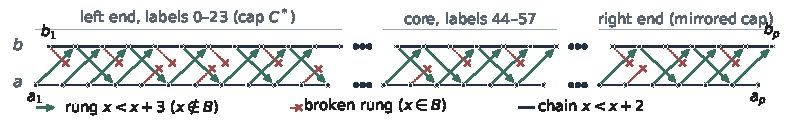
\includegraphics[width=\linewidth]{ladder.pdf}
\caption{The generating relations of $P_2$ ($n=148$) in three windows. The element with label $x$ is drawn at horizontal position $x/2$: even labels form the $a$-chain $a_1<a_2<\cdots$ (bottom), odd labels the $b$-chain (top), so the chains are staggered. Arrows are the cross-chain relations $x<x+3$, i.e.\ $a_r<b_{r+1}$ and $b_r<a_{r+2}$, present when $x\notin B$; dashed stubs marked $\times$ are broken rungs $x\in B$. There is no relation between $a_r$ and $b_r$; in particular $a_1=0$ and $b_1=1$ are incomparable.}
\label{fig:ladder}
\end{figure}

\begin{definition}
Fix $m\ge0$, put $n=108+20m$ and $p=n/2=54+10m$. Let
\[
C^*=\{1,5,8,9,12,13,17,20,21,25,28,29,33,36,39,43\},
\]
\[
I_m=\{\,j: 44\le j\le 52+10m,\ j\bmod 10\in\{3,6,9\}\,\},
\]
and set $B=C^*\cup I_m\cup(n-4-C^*)\cup(n-4-I_m)$. The poset $P_m$ has ground set $\{0,1,\dots,n-1\}$. Its order is the reflexive--transitive closure of the relations
\[
i<i+2\quad(0\le i,\ i+2<n),\qquad i<i+3\quad(i\notin B,\ i+3<n).
\]
\end{definition}

The relations $i<i+2$ make the even labels a chain $a_1<\dots<a_p$ (with $a_r=2r-2$) and the odd labels a chain $b_1<\dots<b_p$ (with $b_r=2r-1$). Adjacent labels are incomparable, so $P_m$ has width exactly two. The relations $i<i+3$ are the \emph{rungs}; in chain notation they read $a_r<b_{r+1}$ (from $i=2r-2$) and $b_r<a_{r+2}$ (from $i=2r-1$). A label in $B$ is a \emph{broken rung}. The set $B$ is invariant under $j\mapsto n-4-j$, so $x\mapsto n-1-x$ is an order-reversing involution of $P_m$ that swaps the two chains. In the interior, the broken rungs are periodic with period $10$ in the labels (period $5$ along each chain), as in Chen's family, whose limit lies in the same field $\mathbb{Q}(\sqrt{6697})$. The end caps $C^*$ and $n-4-C^*$ are what distinguish $P_m$. Figure~\ref{fig:ladder} shows the actual relations.

\begin{lemma}[membership in $\Wdag$]\label{lem:wdag}
For every $m\ge0$, the poset $P_m$ lies in $\Wdag$ and is indecomposable (not a nontrivial ordinal sum).
\end{lemma}
\begin{proof}
Adjacent labels $i$ and $i+1$ are incomparable for every $i$, so the incomparability graph contains the path $0$--$1$--$\cdots$--$(n-1)$ and is connected. A nontrivial ordinal-sum decomposition would disconnect the incomparability graph between summands. Hence $P_m$ is indecomposable, and in particular is not built from singletons and three-element equality cases.
\end{proof}

\subsection*{Lattice paths}
An order ideal of $P_m$ consists of the first $i$ elements of the $a$-chain and the first $j$ elements of the $b$-chain. We identify it with the grid point $(i,j)$, $0\le i,j\le p$, and call it \emph{valid} if it is an ideal. Linear extensions correspond bijectively to monotone unit-step paths from $(0,0)$ to $(p,p)$ through valid points (Figure~\ref{fig:lattice}); the step from row $i-1$ to row $i$ places $a_i$.

\begin{lemma}[local masks and the row word]\label{lem:band}
The following hold for every $m\ge0$.
\begin{enumerate}
\item No two elements of $B$ differ by $2$.
\item A grid point $(i,j)$ with $0\le i,j\le p$ is valid if and only if
\[
-3\le j-i\le 2,\qquad j-i=2\Rightarrow 2i\in B,\qquad j-i=-3\Rightarrow 2i-5\in B .
\]
Equivalently, row $i$ is described by the mask
\[
S_i=\{d\in\{-3,\dots,2\}:\ 0\le i+d\le p,\ \ d=2\Rightarrow 2i\in B,\ \ d=-3\Rightarrow 2i-5\in B\}.
\]
\item The sequence $(S_0,\dots,S_p)$ equals
\[
\mathrm{PRE}\cdot X^m\cdot\mathrm{MID}\cdot X^m\cdot\mathrm{SUF},\qquad |\mathrm{PRE}|=22,\ |X|=5,\ |\mathrm{MID}|=11,\ |\mathrm{SUF}|=22,
\]
with $55+10m=p+1$ rows; the five words are listed in full in Appendix~\ref{app:data}.
\end{enumerate}
\end{lemma}

\begin{proof}
(1) is a direct check of the definition (Lean: \texttt{Structure.broken\_no\_two}). For (2), the chain relations are automatic for prefixes, so $(i,j)$ fails to be an ideal exactly when some rung has its top inside and its bottom outside. The rung $a_{r+1}<b_{r+2}$ (label $2r\notin B$) is violated iff $j\ge r+2$ and $i\le r$; the rung $b_{s+1}<a_{s+3}$ (label $2s+1\notin B$) is violated iff $i\ge s+3$ and $j\le s$. Suppose $(i,j)$ is valid. If $j-i\ge3$, the rungs with $r=i$ and $r=i+1$ would both be violated unless broken, so $2i,2i+2\in B$, two broken labels at distance $2$, contradicting~(1). Hence $j-i\le2$, and if $j-i=2$ the rung with $r=i$ forces $2i\in B$. Symmetrically, if $i-j\ge4$, the rungs with $s=j$ and $s=j+1$ force $2j+1,2j+3\in B$, again contradicting~(1). Hence $i-j\le3$, and only for $i-j=3$ is there a constraint: the rung with $s=j$ forces $2j+1\in B$, and $2j+1=2i-5$ in this case. Conversely, assume the conditions. A violated rung of the first kind needs $i\le r\le j-2$, so $j-i=2$ and $r=i$, but then $2i\in B$ and the rung is absent; a violated rung of the second kind needs $j\le s\le i-3$, so $i-j=3$ and $s=j$, but then $2j+1=2i-5\in B$. (Rungs leaving the ground set near the top are absent, which is consistent with the bounds $0\le i,j\le p$.) This is the Lean theorem \texttt{Structure.valid\_iff\_local}.

For (3), write $\mk{O}=\{-2,-1,0,1\}$, $\mk{R}=\mk{O}\cup\{2\}$, $\mk{L}=\mk{O}\cup\{-3\}$, $\mk{T}=\mk{O}\cup\{-3,2\}$. For $3\le i\le p-2$ the bounds in~(2) are inactive, so $S_i$ is $\mk{O}$, $\mk{R}$, $\mk{L}$ or $\mk{T}$ according as neither, only $2i$, only $2i-5$, or both lie in $B$. The rows $0,1,2$ and $p-1,p$ are clipped by the bounds. Let $R_m=\{j: 33\le j\le 52+10m,\ j\bmod10\in\{3,6,9\}\}$. Since $C^*\cap[33,43]=\{33,36,39,43\}$ follows the same residue pattern,
\[
B\cap[33,\,71+20m]=R_m\cup(n-4-R_m),
\]
and $n-4-R_m$ consists of the labels in $[52+10m,71+20m]$ with residue in $\{1,5,8\}$ mod $10$.
\begin{itemize}
\item \emph{Left cap} (rows $0$--$21$): the labels $2i\le42$ and $2i-5\le37$ meet $B$ only in $C^*$, so $\mathrm{PRE}$ does not depend on $m$.
\item \emph{Left periodic segment} (rows $22+5k+t$, $0\le k<m$, $0\le t<5$): the labels $2i\equiv4+2t$ and $2i-5\equiv9+2t \pmod{10}$ lie in $[39,42+10m]$, where $B$ is the residue set $\{3,6,9\}$. Hence the mask depends only on $t$; it is $\mk{L},\mk{R},\mk{L},\mk{O},\mk{O}$ for $t=0,\dots,4$, which is $X$.
\item \emph{Central seam} (rows $22+5m$ to $32+5m$): the labels lie in $[39+10m,64+10m]$, around the centre $52+10m$ of the reflection $j\mapsto n-4-j$. There $B$ is the residue set $\{3,6,9\}$ below the centre and $\{1,5,8\}$ above it; shifting by $10m$ shows that $\mathrm{MID}$ does not depend on $m$.
\item \emph{Right periodic segment} (rows $33+5m+5k+t$): now $2i\equiv6+2t$ and $2i-5\equiv1+2t\pmod{10}$, tested against $\{1,5,8\}$, which again gives $\mk{L},\mk{R},\mk{L},\mk{O},\mk{O}$.
\item \emph{Right cap} (rows $33+10m$ to $p$): the labels lie in $[61+20m,n]$, where $B$ coincides with $n-4-C^*$, a translate by $20m$ of the case $m=0$; the clipping at $p$ shifts with it. So $\mathrm{SUF}$ does not depend on $m$.
\end{itemize}
The Lean theorems \texttt{mask\_pre}, \texttt{mask\_left}, \texttt{mask\_mid}, \texttt{mask\_right}, \texttt{mask\_suf} and \texttt{row\_word} prove exactly this decomposition for all $m$. Independently, for $m\le1$ we compared the word with the ideals computed by brute force from the generating relations.
\end{proof}

\begin{figure}[t]
\centering
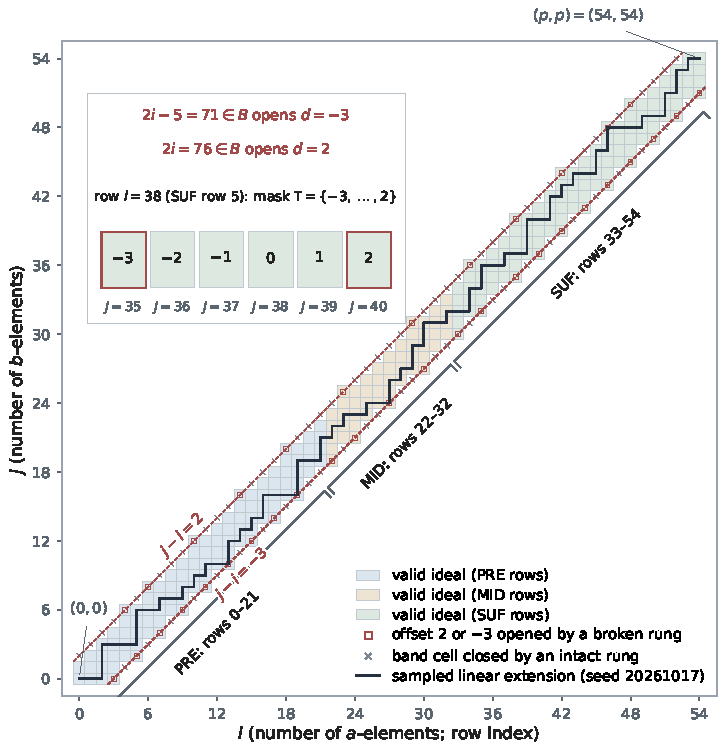
\includegraphics[width=0.76\linewidth]{lattice.pdf}
\caption{The ideal lattice of $P_0$ ($m=0$, $n=108$, $p=54$), computed from the generating relations. A cell is drawn at $(i,j)$ exactly when $\{a_1,\dots,a_i\}\cup\{b_1,\dots,b_j\}$ is an order ideal; the $252$ such points agree with the row masks of Lemma~\ref{lem:band}. Shading gives the row groups $\mathrm{PRE}$ (rows $0$--$21$), $\mathrm{MID}$ ($22$--$32$) and $\mathrm{SUF}$ ($33$--$54$). For $m=0$ the word has no $X$ blocks; for $m\ge1$ each $X^m$ inserts $5m$ rows after $\mathrm{PRE}$ and after $\mathrm{MID}$. Dashed lines: $j-i=2$ and $j-i=-3$. Red squares: extreme offsets opened by a broken rung ($d=2$ iff $2i\in B$, $d=-3$ iff $2i-5\in B$). Crosses: cells of the band that are not ideals because the rung is intact. At $m=0$ every row belongs to a cap or the seam. Black path: one uniformly random linear extension (exact path counts, fixed seed). Inset: the mask of row $i=38$ ($\mathrm{SUF}$ row $5$), $\mk{T}=\{-3,\dots,2\}$, opened at both ends by $71,76\in B$.}
\label{fig:lattice}
\end{figure}

\subsection*{From masks to transfer matrices}
Let $G(i,j)$ be the number of valid paths from $(i,j)$ to $(p,p)$. Then $G(p,p)=1$; for every other valid point,
\[
G(i,j)=G(i+1,j)+G(i,j+1),
\]
where a term is $0$ if its point is invalid or outside the grid; and $G(i,j)=0$ at invalid points. Index the six offsets by $\mathrm{OFF}=(-3,-2,-1,0,1,2)$. A mask $S\subset\mathrm{OFF}$ determines a $6\times6$ integer matrix $\Phi(S)$ that maps $\bigl(G(i+1,i+1+d')\bigr)_{d'\in\mathrm{OFF}}$ to $\bigl(G(i,i+d)\bigr)_{d\in\mathrm{OFF}}$. Processing offsets in decreasing order,
\[
\Phi(S)_{d,\bullet}=
\begin{cases}
0,& d\notin S,\\
e_{d-1}+\text{(row for $d+1$, if present)},& d\in S,
\end{cases}
\]
where $e_{d-1}$ is the standard basis row for offset $d-1$ when $d-1\in\mathrm{OFF}$ (the term $G(i+1,i+d)$), and the second summand is the expression already computed for $G(i,i+d+1)$.

\paragraph{Boundary data from a row word.} The following applies verbatim to all three families. For a word $W=S_1\cdots S_k$ write $\Phi(W)=\Phi(S_1)\cdots\Phi(S_k)$, and let $e_d$ be the basis vector of offset $d$. For a row word $\mathrm{PRE}\cdot X^m\cdot\mathrm{MID}\cdot X^m\cdot\mathrm{SUF}$ put
\[
A=\Phi(X),\quad M=\Phi(\mathrm{MID}),\quad u_E=e_0^{\mathsf T}\Phi(\mathrm{PRE}),\quad u_N=e_0^{\mathsf T}\,\Phi_N(S_0)\,\Phi(\mathrm{PRE}'),\quad v=\Phi(\mathrm{SUF})\,e_{-1}.
\]
Here $e_0^{\mathsf T}$ reads off $G(0,0)$ in row $0$. The vector $e_{-1}$ supplies the seed: in row $p$ the term $e_{d-1}$ with $d=0$ refers to the virtual entry $G(p+1,p)$, which is set to $1$, so that $G(p,p)=1$. $\mathrm{PRE}'$ is $\mathrm{PRE}$ without its first mask $S_0$, and $\Phi_N(S_0)$ keeps only the columns of $\Phi(S_0)$ of offset $\ge0$. These are the crossings of row $0$ at height $h\ge1$, i.e.\ the extensions in which $b_1$ precedes $a_1$. Multiplying along the word gives
\[
E_m=u_E\,A^m M A^m\,v,\qquad N_m=u_N\,A^m M A^m\,v,
\]
where $N_m$ is the number of linear extensions in which $b_1$ precedes $a_1$, the minority event at the \emph{bottom} endpoint. (For $\beta$ the words are taken in the checker's reflected coordinates, Section~\ref{sec:bg}, where the target is again the bottom pair.) For $\alpha$ the periodic block is $X_\alpha=\mk{L}\,\mk{R}\,\mk{L}\,\mk{O}\,\mk{O}$ (rows $22+5k+t$, $t=0,\dots,4$; Lemma~\ref{lem:band}), and

\[
A=\begin{pmatrix}
15&42&69&69&0&0\\ 15&42&69&69&0&0\\ 15&42&69&69&0&0\\ 8&23&38&38&0&0\\ 3&9&15&15&0&0\\ 0&0&0&0&0&0
\end{pmatrix}.
\]
The matrix $M$ and the vectors $u_E,u_N,v$ for $\alpha$ are in Appendix~\ref{app:data} and in~\cite{repo} (\texttt{lean/OneThird/Certificate.lean}). The values of $E_m,N_m$ for $m=0,1,2$ are listed there as well, and $N_0/E_0-\alpha\approx1.07\times10^{-17}$. Already the single $108$-element poset $P_0$ satisfies $\delta(P_0)=N_0/E_0<c_P$.

\subsection*{Spectral structure and the limit}
The characteristic polynomial of $A$ is $z^4(z^2-164z+27)$, and in fact $A^3-164A^2+27A=0$. Its nonzero eigenvalues are $r,s=82\pm\sqrt{6697}$, with $rs=27$. Under $X\mapsto AXA$, the matrix $M$ is annihilated by
\[
q(z)=(z-27)(z^2-26842z+729)=z^3-26869z^2+725463z-19683 ,
\]
that is, $A^3MA^3=26869\,A^2MA^2-725463\,AMA+19683\,M$. Consequently $E_m$ and $N_m$ both satisfy
\[
x_{m+3}=26869\,x_{m+2}-725463\,x_{m+1}+19683\,x_m\qquad(m\ge0).
\]
The dominant root of $q$ is $\rho=r^2=13421+164\sqrt{6697}$. Writing $E_m=c_E\rho^m+O(27^m)$ and $N_m=c_N\rho^m+O(27^m)$ with $c_E>0$ and simplifying exactly in $\mathbb{Q}(\sqrt{6697})$ gives $c_N/c_E=\alpha$.

\paragraph{A unified limit formula.} Let $A$ be any of the three period blocks; each satisfies $A^3-164A^2+27A=0$ (checked exactly). Put
\[
\Pi_r=\frac{A(A-sI)}{r(r-s)},\qquad \Pi_s=\frac{A(A-rI)}{s(s-r)}.
\]
Then $A\Pi_r=r\Pi_r$, $A\Pi_s=s\Pi_s$ and $A=r\Pi_r+s\Pi_s$, so $A^m=r^m\Pi_r+s^m\Pi_s$ for $m\ge1$. Since $0<s<r$,
\[
\frac{E_m}{r^{2m}}\to u_E\Pi_rM\Pi_rv,\qquad \frac{N_m}{r^{2m}}\to u_N\Pi_rM\Pi_rv,\qquad
\lim_{m\to\infty}\frac{N_m}{E_m}=\frac{u_N\,\Pi_r\,M\,\Pi_r\,v}{u_E\,\Pi_r\,M\,\Pi_r\,v},
\]
whenever the denominator is nonzero; it is in fact positive (Corollary~\ref{cor:cp}). This single formula gives $\alpha$, $\beta$ and $\gamma$ from the boundary data of the respective row words; \texttt{certificates/limits\_and\_cP.py} checks the three identities exactly in $\mathbb{Q}(\sqrt{6697})$. The periodic core fixes $r$ and $\Pi_r$; the caps and the seam enter only through $u_E,u_N,M,v$, and since $\Pi_r$ has rank one, $M$ and $v$ cancel as well (Corollary~\ref{cor:rankone}). The approach is from above for every $m$. Since $A^3-164A^2+27A=0$ and $z(z-r)(z-s)$ has distinct roots, $A$ is diagonalizable with eigenvalues among $r,s,0$, and $A^m=r^m\Pi_r+s^m\Pi_s$ for $m\ge1$, where $\Pi_s=(A^2-rA)/(s(s-r))$. Expanding $E_m$ and $N_m$ and using $rs=27$, the coefficient of $r^{2m}$ in $N_m-\alpha E_m$ vanishes by the limit formula, which leaves
\[
N_m-\alpha E_m=C\,27^m+D\,s^{2m},\qquad C=u\,(\Pi_rM\Pi_s+\Pi_sM\Pi_r)\,v,\quad D=u\,\Pi_sM\Pi_s\,v,\quad u=u_N-\alpha u_E .
\]
The identity also holds at $m=0$. For $\alpha$ one gets $C=727011288/\sqrt{6697}$ and $D\approx0.40235$, both positive, so $N_m/E_m>\alpha$ for every $m\ge0$ because $E_m>0$. The ratio of successive errors $(N_{m+1}/E_{m+1}-\alpha)/(N_m/E_m-\alpha)$ tends to $27/r^2\approx1.006\times10^{-3}$. Numerically, $N_m/E_m-\alpha\approx1.07\times10^{-17}$, $1.08\times10^{-20}$, $1.08\times10^{-23}$ for $m=0,1,2$. The same holds for $\beta$ and $\gamma$ (again $C,D>0$). \texttt{certificates/limits\_and\_cP.py} checks these identities and signs exactly.

\paragraph{Method relative to Sah.}
The core and its recurrence are Chen's: for his family Chen proved $E(m+10,n+10)=164\,E(m+5,n+5)-27\,E(m,n)$~\cite[Lemma~15]{Chen18}, with characteristic polynomial $t^2-164t+27$, the same as the nonzero part of the characteristic polynomial of $A$. Sah proved all-pairs dominance for his infinite family by recursive sequences, a finite classification of positions and recurrence inequalities~\cite{Sah21}. Transfer-type counting and dominance uniform in the size parameter are therefore not new. What is new here is: (i)~end caps that push the limit below the published finite value $c_P$; (ii)~a reduction of the all-$m$ dominance question for these caps to finitely many exact certificates; (iii)~for $P_m$, a Lean formalization that starts from the generating relations of the poset.

\section{All-pairs dominance}\label{sec:dominance}

The limit only concerns the pair $(a_1,b_1)$. To show $\delta(P_m)=N_m/E_m$, one must prove that no other pair is more balanced, uniformly in $m$. The argument has four steps: pair events become masked transfer products; a two-generator lemma reduces each position class, for all large exponents at once, to finitely many exact sign checks; a finite classification of positions covers every pair of every member; and small $m$ are checked on the full ideal grid. The primary machine checks (the Lean kernel for $\alpha$, the certificate checkers for $\beta,\gamma$) implement the tail step with rational interval enclosures instead; that path and its relation to the lemma are described at the end of the section.

\subsection*{Pair events as edge insertions}
For $1\le i,j\le p$, let $H_m(i,j)$ be the number of linear extensions with $a_i$ before $b_j$. Every path crosses from row $i-1$ to row $i$ by exactly one horizontal edge, at some height $h$, and $a_i<b_j$ holds exactly when $h<j$. Therefore $H_m(i,j)$ is obtained from the product for $E_m$ by replacing the row-$(i-1)$ matrix with a copy whose columns of offset $\ge j-i$ are set to zero. Since valid offsets lie in $[-3,2]$, only the cutoffs $d=j-i\in\{-3,\dots,3\}$ need checking; $d=-3$ gives $H=0$ and $d=3$ gives $H=E$ (both trivially fine). Pairs inside one chain are comparable.

\subsection*{A finite verification lemma}
\begin{lemma}[finite verification lemma]\label{lem:finite}
Let $A$ be a real square matrix and let $0<s<r$ be real numbers. Fix an integer $K\ge1$ and put $\Lambda=A^2-sA$. Assume:
\begin{enumerate}
\item[(a)] the minimal polynomial of $A$ divides $z(z-r)(z-s)$, i.e.\ $A(A-rI)(A-sI)=0$; so every eigenvalue of $A$ is $0$, $r$ or $s$.
\item[(b)] $E(Y_1,\dots,Y_\ell)$ and $H(Y_1,\dots,Y_\ell)$ are real-valued and linear in each matrix argument $Y_j$ separately, for instance $u\,W_0Y_1W_1\cdots Y_\ell W_\ell\,v$ with fixed vectors $u,v$ and fixed matrices $W_i$.
\item[(c)] A cut $c\in(0,1)$ and one \emph{side} are fixed, giving the linear form $D=cE-H$ (side $H$) or $D=H-(1-c)E$ (side $E-H$).
\item[(d)] $E(Z)>0$ and $D(Z)>0$ for each of the $2^\ell$ tuples $Z=(Z_1,\dots,Z_\ell)\in\{\Lambda,A^K\}^\ell$, with the same side for all tuples.
\end{enumerate}
Then for all exponents $k_1,\dots,k_\ell\ge K$, with $Y_j=A^{k_j}$, we have $E(Y)>0$ and $D(Y)>0$. Hence $H(Y)/E(Y)<c$ (side $H$) or $1-H(Y)/E(Y)<c$ (side $E-H$), so the balance $\min\{H/E,1-H/E\}$ is $<c$ for every such choice of exponents.

In our application $r,s=82\pm\sqrt{6697}$ (so $r+s=164$, $rs=27$, and $s>0$ because $82^2=6724>6697$), and~(a) reads $A^3-164A^2+27A=0$.
\end{lemma}

\begin{proof}
\emph{The identity.} By~(a), $A\Lambda-r\Lambda=A(A-rI)(A-sI)=0$, so $A\Lambda=r\Lambda$. Hence $A^{K+1}-sA^K=A^{K-1}\Lambda=r^{K-1}\Lambda$. We claim that for every $k\ge K$
\[
A^k=\lambda_k\Lambda+\mu_kA^K,\qquad \lambda_k=\frac{r^k-r^Ks^{k-K}}{r(r-s)},\qquad \mu_k=s^{k-K}.
\]
For $k=K$ this holds with $\lambda_K=0$ and $\mu_K=1$. If it holds for $k$, then
$A^{k+1}=\lambda_kr\Lambda+\mu_k\bigl(r^{K-1}\Lambda+sA^K\bigr)$, and $r\lambda_k+s^{k-K}r^{K-1}=\lambda_{k+1}$, $s\mu_k=\mu_{k+1}$.

\emph{Signs.} Since $0<s<r$, $\lambda_k=r^{K}(r^{k-K}-s^{k-K})/(r(r-s))\ge0$ and $\mu_k>0$. This is the only place where the sign of $s$ enters. If $s<0$, the same identity holds but $\mu_k=s^{k-K}$ alternates in sign, so this particular decomposition into $\Lambda$ and $A^K$ no longer has nonnegative coefficients. That does not rule out other nonnegative two-matrix representations. For example, $A=\mathrm{diag}(2,-1)$ satisfies $A^k=\tfrac{2^k-4(-1)^k}{6}A+\tfrac{2^k+2(-1)^k}{6}A^2$ with nonnegative coefficients for all $k\ge1$. Other generator choices need a separate analysis.

\emph{Expansion.} Substitute $Y_j=\lambda_{k_j}\Lambda+\mu_{k_j}A^K$ and expand using linearity in each argument:
\[
E(Y)=\sum_{Z}w_Z\,E(Z),\qquad H(Y)=\sum_Z w_Z\,H(Z),\qquad w_Z=\prod_{j=1}^{\ell}\begin{cases}\lambda_{k_j},&Z_j=\Lambda,\\ \mu_{k_j},&Z_j=A^K.\end{cases}
\]
All weights are $\ge0$, and $w_{(A^K,\dots,A^K)}=\prod_j\mu_{k_j}>0$. Since $c$ does not depend on the exponents, $D$ is a fixed linear combination of $E$ and $H$, so $D(Y)=\sum_Zw_ZD(Z)$ with the same weights. A nonnegative combination of positive numbers with at least one positive weight is positive, so $E(Y)>0$ and $D(Y)>0$.

\emph{Denominator and side.} The hypothesis $E(Z)>0$ gives $E(Y)>0$, so the division by $E$ is legitimate. Because the side is fixed across all $2^\ell$ tuples, the conclusion holds with the same minority direction for all exponents. A case in which some tuples pass only for $H$ and others only for $E-H$ would prove nothing, and the implementation rejects it.
\end{proof}

\paragraph{Scope.} The lemma depends on the special spectral structure of the period block: exactly two nonzero eigenvalues, both positive. Bounded band width, fixed caps and periodicity alone do not provide this. For another periodic core, the nonzero spectrum could contain negative or nonreal eigenvalues, or more than two eigenvalues; then the lemma does not apply as stated, and whether some other choice of generators works must be checked case by case. Sah handled the uniform step for his family through recursions for the counts, a finite classification of positions and recurrence inequalities~\cite{Sah21}. Lemma~\ref{lem:finite} is a different way to organize this step, tailored to the present cores. We do not claim that it is more general than Sah's approach.

\subsection*{Positions and coverage}
\emph{Positions.} Fix a tail threshold $K$ ($K=4$ for $\alpha$) and $m\ge2K$. The insertion of $a_i$ uses row $i-1$, so the insertion rows are $0,\dots,p-1$: all $22$ rows of $\mathrm{PRE}$, all $11$ of $\mathrm{MID}$, and the first $21$ of the $22$ rows of $\mathrm{SUF}$ (row $p$ is only the seed). An insertion row inside a repeated region sits in a block with $k$ complete blocks before it and $l$ after it in that region, where $k+l+1=m$; the block splits as $A^k\cdot(\text{masked block})\cdot A^l$. Since $m\ge2K$, $k$ and $l$ cannot both be $<K$. So, for $K=4$, the nine regimes $(k,l)\in\{(0,\infty),\dots,(3,\infty),(\infty,0),\dots,(\infty,3),(\infty,\infty)\}$, where $\infty$ means ``any exponent $\ge4$'', cover every repeated row (Lean: \texttt{block\_regime\_coverage}, \texttt{row\_region\_coverage}). Short exponents are kept as fixed exact matrices. In the finite regions both repeated segments are long.

\emph{Counting.} The finite regions give $(22+11+22-1)\cdot7-2=54\cdot7-2=376$ checks, the $-2$ being the two endpoint cutoffs ($d=0$ at row $0$, the pair $(a_1,b_1)$, and $d=0$ at row $p-1$, the pair $(a_p,b_p)$). The repeated regions give $2\cdot5\cdot7\cdot9=630$ checks: two regions, five positions per block, seven cutoffs and nine regimes. In total there are $1{,}006$ checks (Lean: \texttt{checked\_case\_count}). Here and below a \emph{check} is one class (position, cutoff and, in the repeated regions, regime). Each class is a single statement for all exponents in it, and it is verified by $2^\ell$ generator tuples (Lemma~\ref{lem:finite}) or by a sequence of interval operations (the interval path).

\emph{Applying the lemma.} In each case $E$ and $H$ are products $u\cdots v$ in which every long repeated segment contributes exactly one factor $A^{k_j}$, so they are multilinear in the $\ell\le3$ long powers, and Lemma~\ref{lem:finite} applies with $c=1743/5000$, or with the finer cut for the $\beta$ endpoint separation. Every value $E(Z)$, $D(Z)$ lies in $\mathbb{Q}(\sqrt{6697})$, and its sign is decided by an integer squared comparison. With $K=4$ this covers $m\ge8$ for $\alpha$, and with $K=8$ it covers $m\ge16$ for $\beta,\gamma$. Hypothesis~(a) holds for the period block $A$ of all three families; the script checks it exactly before use. The identity $A^k=\lambda_k\Lambda+\mu_kA^K$ was also verified symbolically for $1\le K\le5$, $K\le k\le K+7$.

\emph{Small sizes.} For $m=0,\dots,7$ ($\alpha$; $m\le15$ for $\beta,\gamma$), the full $(p+1)\times(p+1)$ ideal grid is built directly from the generating relations, without assuming the band structure, and exact integer path counts are compared pair by pair with the transfer formula.

\subsection*{The two endpoints and the result}
Both verification paths certify that every non-endpoint pair has balance below $1743/5000=0.3486$; the largest certified upper bound among the $1{,}006$ interval cases is $\approx0.348574697077$, at row $3$ with cutoff $-1$, that is, the pair $(a_4,b_3)$ (and at its mirror image). A separate interval enclosure gives $0.34884<N_m/E_m<\tfrac12$ for all $m\ge8$. The reflection $x\mapsto n-1-x$ maps the event $\{b_1<a_1\}$ to the corresponding event for the top pair $(a_p,b_p)$, so the two endpoint pairs tie exactly. Hence:

\begin{proposition}\label{prop:dom}
For every $m\ge0$, the pairs $(a_1,b_1)$ and $(a_p,b_p)$ both have balance $N_m/E_m>0.34884$, and every other pair of $P_m$ has balance $<0.3486$. Hence $\delta(P_m)=N_m/E_m$, and the maximizing pair is not unique.
\end{proposition}

\begin{corollary}[every member lies below $c_P$]\label{cor:cp}
For each of the families $\alpha$ ($P_m$), $\beta$ and $\gamma$ of Section~\ref{sec:bg}, and every $m\ge0$, the $m$-th member $Q$ satisfies $\delta(Q)<c_P=1087457557/3117322468$.
\end{corollary}
\begin{proof}
By all-pairs dominance (Proposition~\ref{prop:dom} for $\alpha$, Section~\ref{sec:bg} for $\beta,\gamma$), $\delta(Q)=N_m/E_m$ with $E_m=u_EA^mMA^mv$ and $N_m=u_NA^mMA^mv$ as in Section~\ref{sec:family}. For $m\ge1$ apply Lemma~\ref{lem:finite} with $K=1$, $\ell=2$, $Y_1=Y_2=A^m$, side $H$ with $H=N$, and $c=c_P$. Its hypotheses are $E(Z)>0$ and $1087457557\,E(Z)-3117322468\,N(Z)>0$ for the four tuples $(Z_1,Z_2)\in\{\Lambda,A\}^2$, where $E(Z)=u_EZ_1MZ_2v$ and $N(Z)=u_NZ_1MZ_2v$. These are eight sign conditions in $\mathbb{Q}(\sqrt{6697})$. For $m=0$ the inequality $1087457557\,E_0>3117322468\,N_0$ is checked in integers. All checks pass for all three families (\texttt{certificates/limits\_and\_cP.py}). The tuple $(\Lambda,\Lambda)$ also shows that the denominator of the unified limit formula is positive.
\end{proof}

\begin{remark}[the two-generator reformulation; suggested by GPT 6 Pro]\label{rem:twogen}
Lemma~\ref{lem:finite} and its use above are the reformulation suggested by GPT 6 Pro. It is implemented in \texttt{certificates/two\_generator\_check.py} of~\cite{repo}, which passes all $1{,}006$ non-endpoint cases for $\alpha$ ($K=4$), all $2{,}056$ for each of $\beta,\gamma$ ($K=8$), and the $\beta$ other-endpoint separation, which is one further class (so the $\beta$ count including it is $2{,}057$, as in Section~\ref{sec:bg}). The generator $\Lambda=A^2-sA$ is $r(r-s)\Pi_r$, a multiple of the spectral projector in the unified limit formula of Section~\ref{sec:family} (and $\Pi_r=P$ in the interval enclosure below).
\end{remark}

\subsection*{Interval certificates and the Lean check}
The Lean development and the $\beta,\gamma$ checkers do not use Lemma~\ref{lem:finite}; they enclose the long powers. Put $t=s/r\in(0,1)$. There are matrices $P,Q$ over $\mathbb{Q}(\sqrt{6697})$ with
\[
AP=rP,\qquad AQ=sQ,\qquad P+Q=A/r ,
\]
so $A^k/r^k=P+t^{k-1}Q$ for every $k\ge1$. We enclose $\sqrt{6697}$ between consecutive rationals with denominator $10^{40}$ (checked by integer squaring) and round outward to the mesh $10^{-30}$: lower endpoints are rounded down and upper endpoints up, with exact floor/ceiling on rationals. This yields one rational interval matrix $\mathcal T$ that contains $A^k/r^k$ for every $k\ge4$.

\emph{Normalization.} Every long power $A^k$ is replaced by $A^k/r^k\in\mathcal T$. The same positive factor $r^k$ divides $H$ and $E$, so the ratio $H/E$ is unchanged. Short powers ($k\le3$) are kept exact. The positions, regimes and $1{,}006$ cases are those above.

\emph{Each check.} Interval matrix products give rational enclosures $[H^-,H^+]$ and $[E^-,E^+]$. The check first requires $E^->0$ (a positive denominator lower bound) and then one of
\[
5000\,H^+<1743\,E^- \quad(\text{so }H/E<\tfrac{1743}{5000})
\qquad\text{or}\qquad
3257\,E^+<5000\,H^- \quad(\text{so }1-H/E<\tfrac{1743}{5000}),
\]
which fixes which of $H$ and $E-H$ is the minority in that case. Appendix~\ref{app:data} shows a near-critical certificate record.

\paragraph{Shared components.} The interval certificates enclose $A^k/r^k=P+t^{k-1}Q$ for all $k\ge K$ in one rational interval matrix and compare rational interval bounds. Lemma~\ref{lem:finite} instead checks exact algebraic signs at $2^\ell$ generator tuples, without intervals. These are different verification paths, but they share components. Both read the same row words: for $\alpha$ the words of \texttt{certificates/alpha/certificate.json}, identical to those in \texttt{Structure.lean}; for $\beta,\gamma$ the \texttt{structure} field of the stored certificates, whose correctness for all $m$ is proved by \texttt{structure.py}. For $\beta,\gamma$ they also share the module \texttt{arithmetic.py}, which provides arithmetic in $\mathbb{Q}(\sqrt{6697})$, matrix products, the map $S\mapsto\Phi(S)$ and column masking. An error in these shared parts would affect both checks. For $\alpha$, the primary check runs in the Lean kernel and shares only the row-word data with the script.


\begin{corollary}[rank-one form of the limit]\label{cor:rankone}
Let $A$ be the period block of $\alpha$, $\beta$ or $\gamma$ (in the coordinates of its row word), $r=82+\sqrt{6697}$, and let $x$, $y$ be right and left eigenvectors, $Ax=rx$ and $y^{\mathsf T}A=ry^{\mathsf T}$. Then $\Pi_r=xy^{\mathsf T}/(y^{\mathsf T}x)$, and
\[
\lim_{m\to\infty}\frac{N_m}{E_m}=\frac{u_N\,x}{u_E\,x}.
\]
One can take
\begin{align*}
x_\alpha&=\Bigl(1,1,1,\tfrac{\sqrt{6697}-44}{69},\tfrac{\sqrt{6697}-67}{69},0\Bigr)^{\mathsf T},\\
x_{\beta,\gamma}&=\Bigl(0,\tfrac{529+7\sqrt{6697}}{61},\tfrac{404+5\sqrt{6697}}{61},\tfrac{279+3\sqrt{6697}}{61},\tfrac{154+\sqrt{6697}}{61},1\Bigr)^{\mathsf T}.
\end{align*}
\end{corollary}
\begin{proof}
The characteristic polynomial of $A$ is $z^4(z^2-164z+27)$, so $r$ is a simple eigenvalue, and by~(a) of Lemma~\ref{lem:finite} $A$ is diagonalizable. Hence $\Pi_r$, the projector onto the $r$-eigenspace along the other eigenspaces, has rank one and equals $xy^{\mathsf T}/(y^{\mathsf T}x)$ (note $y^{\mathsf T}x\ne0$). Substituting into the unified limit formula of Section~\ref{sec:family}, numerator and denominator become $(u_Nx)\,\kappa$ and $(u_Ex)\,\kappa$ with $\kappa=(y^{\mathsf T}Mx)(y^{\mathsf T}v)/(y^{\mathsf T}x)^2$. The denominator is positive (Corollary~\ref{cor:cp}), so $\kappa\ne0$ and $u_Ex\ne0$, and $\kappa$ cancels. The script \texttt{certificates/rank\_one\_limits.py} checks exactly in $\mathbb{Q}(\sqrt{6697})$ that $Ax=rx$, $y^{\mathsf T}A=ry^{\mathsf T}$, $A(A-sI)/(r(r-s))=xy^{\mathsf T}/(y^{\mathsf T}x)$, $u_Ex>0$, and that $(u_Nx)/(u_Ex)$ equals $\alpha$, $\beta$, $\gamma$ respectively.
\end{proof}

\paragraph{Interpretation and scope.} In the coordinates of the row word the target pair sits at the start of the word, so $u_E$ and $u_N$ are determined by the first rows, i.e.\ by the cap next to the target endpoint together with the adjacent part of the core. The asymptotic endpoint probability therefore depends only on that cap and on the principal right eigenvector $x$ of the core; the far cap (through $v$) and the seam (through $M$) cancel in the limit. For $\alpha$ and $\gamma$ the caps are mirror images, so this is the bottom cap. For $\beta$ the checker coordinates are reflected (Section~\ref{sec:bg}), so the surviving cap is the original \emph{right} cap, next to the maximizing top pair; $\beta$ does not depend on the left cap $L$. The corollary says nothing about finite $m$: the far cap and the seam still enter the finite-size corrections of $N_m/E_m$, the balances of all other pairs, and hence all-pairs dominance and the identity of the maximizing pair.

\paragraph{The far endpoint.} For $\beta$ and $\gamma$ the certificates also use, in checker coordinates,
\[
v_{\mathrm{other}}=\Phi(\mathrm{SUF}')\,\Phi_O(S_{p-1})\,\Phi(S_p)\,e_{-1},
\]
where $\mathrm{SUF}'$ is $\mathrm{SUF}$ without its last two masks $S_{p-1},S_p$, and $\Phi_O(S_{p-1})$ keeps only the columns of $\Phi(S_{p-1})$ of offset $\ge0$ (the complement of the masked copy used for $H$ with cutoff $0$, Section~\ref{sec:dominance}). This is the suffix boundary vector with the column mask for the far-end pair event. Hence
\[
O_m=u_E\,A^mMA^m\,v_{\mathrm{other}}=E_m-H_m(p,p)
\]
is the number of linear extensions in which $b_p$ precedes $a_p$ in checker coordinates. Under the reflection $\phi$ of Section~\ref{sec:bg} this is the event that $b_1$ precedes $a_1$ in the original coordinates, i.e.\ the minority event at the original bottom pair. By Corollary~\ref{cor:rankone},
\[
\lim_{m\to\infty}\frac{O_m}{E_m}=\frac{u_E\Pi_rM\Pi_rv_{\mathrm{other}}}{u_E\Pi_rM\Pi_rv}=\frac{y^{\mathsf T}v_{\mathrm{other}}}{y^{\mathsf T}v},
\]
which depends only on the far cap. For $\beta$ this is $\approx0.348843459592846368$, determined by the left cap $L$ alone and below both $\beta$ and the endpoint cut $6976869191857/(2\cdot10^{13})$ of Section~\ref{sec:bg}; $O_m/E_m$ exceeds it by $\approx5.92\times10^{-40}$, $5.95\times10^{-43}$, $5.99\times10^{-46}$ for $m=0,1,2$. For $\gamma$ it equals $\gamma$ exactly, as the tie requires. The script \texttt{rank\_one\_limits.py} rebuilds $v_{\mathrm{other}}$ from the word, checks it against the stored vector, checks the limit formula exactly, and checks $O_m$ for $m=0,1,2$ against a direct count, from the generating relations, of the extensions with $b_1$ before $a_1$.

\paragraph{Example: Chen's cap.} Chen's poset $\mathcal P(5k,5k)$~\cite[Definitions~7--8]{Chen18} is, in our notation, the ladder with $n=10k$ and broken set $\{j\le n-4: j\bmod10\in\{1,5,8\}\}$. By the local-mask rule of Lemma~\ref{lem:band}, its full row word (rows $0,\dots,5k$) is
\[
\mk{a}\,\mk{b}\,\mk{O}\,(\mk{L}\,\mk{R}\,\mk{L}\,\mk{O}\,\mk{O})^{k-1}\,\mk{L}\,\mk{O}\,\mk{z}\qquad(k\ge1),
\]
of length $3+5(k-1)+3=5k+1$; the suffix $\mk{L}\,\mk{O}\,\mk{z}$ is the clipping at the top of the finite grid (for $k=1$ the word is $\mk{a}\mk{b}\mk{O}\mk{L}\mk{O}\mk{z}$). So in the same coordinates its cap at the target end is the three-row prefix $\mk{a}\,\mk{b}\,\mk{O}$, followed by the block $X_\alpha$, with
\[
u_E=(1,3,5,5,0,0),\qquad u_N=(0,1,2,2,0,0).
\]
With the same eigenvector $x_\alpha$, and $\xi=(\sqrt{6697}-44)/69$,
\[
\frac{u_Nx_\alpha}{u_Ex_\alpha}=\frac{3+2\xi}{9+5\xi}=\frac{93-\sqrt{6697}}{32}\approx0.3488999922,
\]
which is Chen's limit. The $22$-row prefix $\mathrm{PRE}$ of $\alpha$ gives $\alpha$ instead. Since the core, $r$ and $x_\alpha$ are the same, the whole difference $\approx5.653\times10^{-5}$ between the two limits comes from the prefix vectors. Both evaluations are exact, and the bottom-pair balance of $\mathcal P(40,40)$, computed directly from the generating relations, agrees with Chen's limit to $13$ digits. The script \texttt{rank\_one\_limits.py} checks all of this, including the full word for $k=1,\dots,8$, both from the local-mask rule and from the order ideals of the generated order.

\section{Lean formalization}\label{sec:lean}

The development is in \texttt{lean/} of~\cite{repo}. It uses Lean~4~\cite{Lean4} (toolchain \texttt{v4.35.0}) and Mathlib~\cite{Mathlib20} at commit \texttt{56a00585}. The formalization follows Sections~\ref{sec:family}--\ref{sec:dominance} and does not trust the Python certificates.

\begin{itemize}
\item \textbf{The poset.} \texttt{familyOrder m} is a \texttt{PartialOrder} on \texttt{Fin (108+20*m)}, defined as the reflexive--transitive closure of the $+2$ and unbroken $+3$ generators, with $B$ exactly as above. Linear extensions are permutations respecting this order. \texttt{Balance6.delta m} is the maximum over incomparable pairs of $\min\{\Prob(x<y),\Prob(y<x)\}$ under the uniform distribution on these extensions.
\item \textbf{Structure and counting.} Lemma~\ref{lem:band} is \texttt{Structure.valid\_iff\_local} and \texttt{Structure.row\_word}. Lean proves a bijection between linear extensions and grid paths, and identifies path counts with the transfer products.
\item \textbf{Dominance.} The $1{,}006$ rational interval cases, the spectral tail enclosure and the eight finite grids ($m<8$) are checked by the kernel using \texttt{decide}; there are no uses of \texttt{native\_decide}.
\item \textbf{Limit.} The kernel checks three things by \texttt{decide}: the values $E_m,N_m$ for $m=0,1,2$, the identity $A^4(A^2-164A+27I)=0$, and the matrix identity $A^3MA^3=26869\,A^2MA^2-725463\,AMA+19683\,M$. Algebraic rewriting turns the last identity into the recurrence $X_{m+3}=26869X_{m+2}-725463X_{m+1}+19683X_m$ for $X\in\{E,N\}$ and all $m\ge0$. The roots of this recurrence are $r^2=13421+164\sqrt{6697}$, $27$ and $s^2$. Over $\mathbb{R}$, Lean proves that each of $E_m$ and $N_m$ equals a three-term closed form $(a+b\sqrt{6697})\,r^{2m}+c\,27^m+(a-b\sqrt{6697})\,s^{2m}$ with explicit rational $a,b,c$. The proof is by uniqueness for the recurrence, with the three initial values matched by \texttt{norm\_num}, \texttt{ring} and \texttt{nlinarith}. Dividing by $r^{2m}$ and using $0\le27/r^2,\,s^2/r^2<1$ gives the limit $(a_N+b_N\sqrt{6697})/(a_E+b_E\sqrt{6697})=\alpha$ (\texttt{ratio\_tendsto} in \texttt{Certificate.lean}).
\end{itemize}

\begin{table}[h]
\centering
{\footnotesize
\begin{tabular}{@{}p{0.42\linewidth}p{0.50\linewidth}@{}}
\toprule
Body claim & Lean name \\
\midrule
Generating relations define a partial order & \texttt{familyOrder} \\
Local validity, row word (Lemma~\ref{lem:band}) & \texttt{Structure.valid\_iff\_local}, \newline\texttt{Structure.row\_word} \\
$|\Lin(P_m)|=E_m$ & \texttt{RowCounts7.extension\_card\_eq\_E} \\
Bottom minority count equals $N_m$ & \texttt{BottomCounts7.bottom\_card\_eq\_N} \\
Pair event equals masked transfer count & \texttt{Counting6.H\_eq\_event\_card}, \newline\texttt{HitRows7.H\_eq\_crossing} \\
$1{,}006$ checked cases & \texttt{CertificateCoverage4.checked\_case\_count} \\
$\delta(P_m)=N_m/E_m$ & \texttt{Balance7.delta\_eq\_ratio} \\
$\delta(P_m)\to\alpha$ & \texttt{Balance7.delta\_tendsto} \\
Width two; $P_m\in\Wdag$; $\alpha<c_P<\sigma_{\mathrm S}$ & paper (Lemma~\ref{lem:wdag}; exact squared comparisons) \\
\bottomrule
\end{tabular}}
\caption{Correspondence between body claims and Lean declarations. The last row is intentionally not a named Lean theorem.}\label{tab:lean}
\end{table}

The main theorems are \texttt{Balance7.delta\_eq\_ratio} and \texttt{Balance7.delta\_tendsto} in \texttt{OneThird/Balance7.lean}. An audit of all $10{,}311$ project declarations shows dependence only on \texttt{propext}, \texttt{Classical.choice} and \texttt{Quot.sound}; no source file contains \texttt{sorry}, \texttt{admit}, \texttt{native\_decide} or a custom axiom. A full \texttt{lake build} exits with code $0$; besides the recorded macOS/arm64 build, we re-ran the build and the complete audit from a fresh clone on Linux x86\_64 with the Lean sources of commit \texttt{6786282}, and the regenerated audit files were byte-identical to the committed ones. The pinned commit \texttt{\pin} has the same Lean declarations; only the header comment of \texttt{Certificate.lean} differs, and that file was rechecked separately. The build and audit procedure is in Appendix~\ref{app:repro}.

\section{Further improvements: the families $\beta$ and $\gamma$}\label{sec:bg}

Changing the caps while keeping the period-$5$ core lowers the limit further. Both families below have $n=248+20m$ and $p=n/2$, the same chain relations $i<i+2$, and rungs $i<i+3$ for $i\notin B$. The core broken set is $\{100\le j\le(n-4)/2: j\bmod10\in\{3,6,9\}\}$ together with its mirror image under $j\mapsto n-4-j$. The connectedness argument of Lemma~\ref{lem:wdag} shows that both families are indecomposable members of $\Wdag$.

\subsection*{Asymmetric caps ($\beta$): a unique maximizer} The left cap is
\[
\begin{aligned}L=\{&1,5,8,9,12,13,17,20,21,25,28,29,33,36,37,43,\\&46,47,50,53,58,64,67,68,73,76,83,89,90,93,96,97\}.\end{aligned}
\]
The right cap is $n-4-R$, where
\[
\begin{aligned}R=\{&1,5,8,9,12,13,17,20,21,25,28,29,33,36,37,\\&45,48,51,55,58,61,62,65,73,76,77,83,89,90,93\}.\end{aligned}
\]
Because the two caps differ, the reflection $x\mapsto n-1-x$ is no longer a symmetry, and the two endpoint pairs no longer tie. The structural point of $\beta$ is that the asymmetric caps produce a \emph{unique} maximizing pair, the top endpoint pair $(a_p,b_p)$. Write $E_m^{\beta}$ for $|\Lin|$ and $N_m^{\beta}$ for the number of extensions with $b_p$ before $a_p$ (the minority at the top endpoint). Then
\[
\begin{aligned}\beta&=\frac{70601103221348402231752613608561321408507-76527504\sqrt{6697}}{202386202979838556018601359840018770821908}\\&\approx0.3488434595928537 .\end{aligned}
\]

\paragraph{Reflection used by the checker.} For a broken set $B\subseteq\{0,\dots,n-4\}$ write $P(B)$ for the ladder above. The map $\phi(x)=n-1-x$ sends the relation $i<i+2$ to $n-3-i<n-1-i$, and the rung $i<i+3$ ($i\notin B$) to $i'<i'+3$ with $i'=n-4-i\notin n-4-B$. Hence $\phi$ is an isomorphism from $P(B)$ to the dual of $P(n-4-B)$. It reverses linear extensions, so $\Prob_{P(B)}(x<y)=\Prob_{P(n-4-B)}(\phi(y)<\phi(x))$ and the balance of every pair is preserved. Since $n$ is even, $\phi$ swaps the chains, with $\phi(a_i)=b_{p+1-i}$ and $\phi(b_j)=a_{p+1-j}$. In particular $\phi$ maps the top pair $(a_p,b_p)$ to the bottom pair $(b_1,a_1)$, and the event $\{b_p<a_p\}$ to $\{b_1<a_1\}$. The $\beta$ checker works with the reflected set \texttt{broken(m, True)}${}=n-4-B$, so its target is the bottom pair $(a_1,b_1)$ and its ``other endpoint'' is the top pair. In these reflected coordinates the row-mask word is $\mathrm{PRE}(53)\,X_{\beta,\gamma}^m\,\mathrm{MID}(11)\,X_{\beta,\gamma}^m\,\mathrm{SUF}(61)$, with the same word structure for $\gamma$. The periodic block is $X_{\beta,\gamma}=\mk{R}\,\mk{L}\,\mk{O}\,\mk{O}\,\mk{L}$, a cyclic shift of $X_\alpha=\mk{L}\,\mk{R}\,\mk{L}\,\mk{O}\,\mk{O}$. Both blocks, and the full words for $m=0,1,2$, were recomputed from the generating relations by testing which prefixes are order ideals. The block matrix is
\[
A_{\beta,\gamma}=\Phi(X_{\beta,\gamma})=\begin{pmatrix}
0&0&0&0&0&0\\ 26&57&88&88&0&0\\ 19&42&65&65&0&0\\ 12&27&42&42&0&0\\ 5&12&19&19&0&0\\ 1&3&5&5&0&0
\end{pmatrix}.
\]
If $A_\alpha=\Phi(\mk{L})\,Y$ with $Y=\Phi(\mk{R}\,\mk{L}\,\mk{O}\,\mk{O})$, then $A_{\beta,\gamma}=Y\,\Phi(\mk{L})$. So the two blocks have the same nonzero spectrum, and indeed $A_{\beta,\gamma}^3-164A_{\beta,\gamma}^2+27A_{\beta,\gamma}=0$ (checked exactly). The boundary data $u_E,u_N,M,v$ are extracted from the word exactly as in Section~\ref{sec:family}; they are listed in Appendix~\ref{app:data}.

Dominance for $\beta$ (in original coordinates) splits into three statements, all certified for every $m\ge0$:
\begin{enumerate}
\item every \emph{non-endpoint} cross-chain pair has balance $<1743/5000=0.3486$;
\item the bottom endpoint $(a_1,b_1)$ has balance $<6976869191857/20000000000000=0.34884345959285$;
\item $N_m^{\beta}/E_m^{\beta}>0.34884345959285$.
\end{enumerate}
Hence $\delta=N_m^{\beta}/E_m^{\beta}$, attained only at $(a_p,b_p)$. A sample record for~(2) is in Appendix~\ref{app:data}.

\subsection*{Symmetric caps ($\gamma$)} Both caps equal
\[
\begin{aligned}C_\gamma=\{&1,5,8,9,12,13,17,20,21,25,28,29,33,\\&36,37,43,49,55,61,67,73,79,85,91,97\},\end{aligned}
\]
the right cap being reflected. Write $E_m^{\gamma}$ and $N_m^{\gamma}$ for $|\Lin|$ and the bottom-endpoint minority count. The two endpoint pairs tie exactly, and
\[
\begin{aligned}\gamma&=\frac{113344761041171128772377413341625230454875-4782969\sqrt{6697}}{324915826638865693871423059126368044433152}\\&\approx0.3488434595928454 .\end{aligned}
\]
Every non-endpoint cross-chain pair has balance $<1743/5000$, so $\delta=N_m^{\gamma}/E_m^{\gamma}$.

\subsection*{Certificates}
\begin{lemma}[row words of $\beta,\gamma$ for all $m$]\label{lem:bgword}
For $\beta$ and for $\gamma$ and every $m\ge0$, the row masks in the checker coordinates form the word $\mathrm{PRE}\,X_{\beta,\gamma}^m\,\mathrm{MID}\,X_{\beta,\gamma}^m\,\mathrm{SUF}$ with $|\mathrm{PRE}|=53$, $|\mathrm{MID}|=11$, $|\mathrm{SUF}|=61$ stored in the certificate.
\end{lemma}
\begin{proof}[Proof (verified by \texttt{structure.py})]
First, no two broken labels differ by $2$. The script checks this inside each of the five pieces of the broken-bit word (left cap, core period, seam, reflected core period, right cap) and across each of the eight possible joins of consecutive pieces, including a repeated period followed by itself; this covers every $m$. The proof of Lemma~\ref{lem:band}(2) uses only this property, so it applies verbatim: the mask of row $i$ is determined by the bounds $0\le i+d\le p$ and by whether $2i$ and $2i-5$ lie in $B$. Next, every row of every member is an instance of one of $135$ affine row classes, with all parameters ranging over the nonnegative integers. A row of $\mathrm{PRE}$ is $i=t$ ($53$ classes); a row of $\mathrm{MID}$ is $i=53+5m+t$ ($11$ classes) and a row of $\mathrm{SUF}$ is $i=64+10m+t$ ($61$ classes). A row in the first repeated region is $i=53+5k+t$ with $m=k+l+1$ ($5$ classes), and a row in the second is $i=69+10k+5l+t$ with $m=k+l+1$ ($5$ classes). Here $k$ and $l$ count the complete periods before and after the row's block, so every row of every $m\ge0$ lies in exactly one class. For each class and each offset $d$, the script evaluates the bounds and the two rung labels as affine forms $f=c_0+\sum_{i=1}^{d'}c_it_i$ in the class parameters $t_i\ge0$. It decides every comparison by one of exactly two criteria (the functions \texttt{nonneg} and \texttt{negative}):
\begin{itemize}
\item[(N)] if $c_i\ge0$ for all $i=0,\dots,d'$, then $f\ge0$ for all parameter values;
\item[(S)] if $c_0<0$ and $c_i\le0$ for all $i\ge1$, then $f<0$ for all parameter values.
\end{itemize}
A branch is entered only when its test, an instance of (N) or (S), holds. When a test fails, the script continues only by \emph{asserting} the criterion for the remaining case: after the out-of-range test (S) fails it asserts (N) for both range bounds; after the two cap tests fail it asserts (N) for both bounds of the core region; and after the seam test $h-j\ge0$ (N) fails it asserts $h-j<0$ by (S). So every branch taken is certified for all parameter values, and a failed assertion would abort. In a cap the label is further asserted to be constant ($c_i=0$ for $i\ge1$), so its membership in $B$ is a fixed lookup; in the core the parameter coefficients of the label are asserted to be multiples of $10$, so its residue modulo $10$, which decides membership in $B$, is constant. Hence each class has a constant mask, and the script checks that it equals the stored mask. The count $135=53+11+61+5+5$ is the number of entries \texttt{affine\_row\_cases} produced by the code and stored in both certificates.
\end{proof}

For both families the method is that of Section~\ref{sec:dominance} with tail threshold $K=8$ (so $2K+1=17$ regimes):
\begin{itemize}
  \item the row word for all $m$ (Lemma~\ref{lem:bgword});
  \item a spectral enclosure covering all $m\ge16$;
  \item full ideal-grid exact dynamic programming for $m=0,\dots,15$, comparing all cross-chain pairs ($667{,}616$ in total for $\gamma$) with the transfer formula.
\end{itemize}
The interval checks (classes in the sense of Section~\ref{sec:dominance}) number $(53+11+61-1)\cdot7-e+2\cdot17\cdot5\cdot7$. Here $e=2$ for $\gamma$ (both endpoint cutoffs are excluded and handled by the tie), giving $2{,}056$, and $e=1$ for $\beta$ (the other endpoint is checked against the finer cut $6976869191857/(2\cdot10^{13})$), giving $2{,}057$. The largest certified non-endpoint upper bound is $\approx0.3485746971005$ in both families. The inequalities $\gamma<\beta<\alpha$ are proved by exact squared comparisons in $\mathbb{Q}(\sqrt{6697})$. The checkers use only Python integers and \texttt{fractions.Fraction}, with no floating point in any decision. They are not formalized in Lean; Remark~\ref{rem:twogen} gives an independent check of the tail part. Commands and implementation details are in Appendix~\ref{app:repro}.

\subsection*{The finite poset $P^\dagger$}
An exact local search started from the $m=0$ member of the $\beta$ family produced a $248$-element ladder $P^\dagger$; the $\gamma$ family was derived from it afterwards (Section~\ref{sec:search}). Let $B^\dagger$ be the union of three blocks: the left cap
$\{1,5,8,9,12,13,17,20,21,25,28,29,33,36,37,43,49,55,61,67,73,79,85,91,97\}$,
the arithmetic progression $103+6k$ for $k=0,\dots,13$ (that is, $\{103,109,\dots,181\}$), and the right block
\begin{lstlisting}[basicstyle=\ttfamily\scriptsize,breaklines=true,breakatwhitespace=true,frame=single,framerule=0.3pt,columns=fullflexible,linewidth=\linewidth]
{186, 189, 193, 196, 199, 202, 203, 207, 208, 211,
 215, 216, 219, 223, 224, 227, 231, 232, 235, 236, 239, 243}
\end{lstlisting}
$P^\dagger$ has ground set $\{0,\dots,247\}$, and its order is generated by $i<i+2$ ($i+2<248$) and $i<i+3$ ($i\notin B^\dagger$, $i+3<248$), with chains $a_r=2r-2$ and $b_r=2r-1$, $1\le r\le124$.

\begin{proposition}[computer-verified, not formalized]\label{prop:dagger}
$P^\dagger$ is an indecomposable member of $\Wdag$, and $\delta(P^\dagger)=N^\dagger/E^\dagger$, where $E^\dagger=|\Lin(P^\dagger)|$ and
\begin{align*}
N^\dagger&=\texttt{\seqsplit{651413227161569890696144661362095442432291791687618240}},\\
E^\dagger&=\texttt{\seqsplit{1867351126266980493055916252346490607551032183835026048}}.
\end{align*}
The maximizing pair is $(a_1,b_1)$, and it is unique: the second largest balance, attained at the top pair $(a_{124},b_{124})$, is smaller by $\approx3.1745\times10^{-14}$. Moreover $\delta(P^\dagger)<\gamma$ (by $\approx7.724\times10^{-37}$), and hence $\delta(P^\dagger)<\beta<\alpha<c_P$.
\end{proposition}
\begin{proof}[Verification]
Membership and indecomposability follow as in Lemma~\ref{lem:wdag}. The script \texttt{certificates/pdagger/verify\_pdagger.py} reads only $B^\dagger$ and the stored $N^\dagger,E^\dagger$ from \texttt{certificates/pdagger/pdagger.json}. It rebuilds the order as the transitive closure of the generating relations and finds all $557$ order ideals $\{a_1,\dots,a_i\}\cup\{b_1,\dots,b_j\}$ by a down-set test. An integer path DP then gives $E^\dagger$ and, for every cross-chain pair, the number of extensions with $a_i$ before $b_j$; comparable pairs are checked to give $0$ or $E^\dagger$. Among the $308$ incomparable cross-chain pairs, the maximum of $\min\{H,E^\dagger-H\}$ is $N^\dagger$, attained only at $(a_1,b_1)$. For $\gamma=(a-b\sqrt{6697})/c$ (Section~\ref{sec:bg}), $\delta(P^\dagger)<\gamma$ is equivalent to $U=aE^\dagger-cN^\dagger>0$ and $U^2-6697\,(bE^\dagger)^2>0$, both checked in integers; the same is done for $\beta$, and $N^\dagger\cdot3117322468<1087457557\cdot E^\dagger$ gives $\delta(P^\dagger)<c_P$. The run takes about $0.2$ seconds. The search-time computation that first found $P^\dagger$ (a different DP implementation) gives the same $N^\dagger,E^\dagger$.
\end{proof}

Thus the strongest \emph{certified finite} upper bound here is $\deltadag\le\delta(P^\dagger)$, while $\gamma$ is the smallest \emph{certified family limit}. No indecomposable periodic-core family with limit below $\gamma$ has been certified in this project. The ordinal sums $Q_k=P^\dagger\oplus C_k$ with a $k$-element chain do lie in $\Wdag$, with $\delta(Q_k)=\delta(P^\dagger)>1/3$; they are not equality cases. They are excluded only from our additional goal of indecomposable families, and they give no new constant and no accumulation point, since $\delta(Q_k)$ is the same rational number for every $k$.

\section{How the constructions were found}\label{sec:search}
No proof depends on this section.

\paragraph{Search space.} All candidates are width-two broken-rung ladders, determined by the broken set $B$. The ``cap, periodic interior, mirror'' framework led to $\alpha$; annealing of two independent end caps around the fixed core gave $\beta$; an exact one- and two-rung local search at $n=248$ gave $P^\dagger$; and $\gamma$ copies the left cap of $P^\dagger$ to both ends. Sizes, schedules, the order of the moves and the origin of the framework are in Appendix~\ref{app:search}.

\paragraph{Scoring and pipeline.} A candidate was always scored by its full balance constant $\delta$ at one fixed finite size, i.e.\ the maximum over all cross-chain pairs, computed by lattice-path dynamic programming (in double precision for the $\alpha$ cap search, with exact recomputation of the selected candidate; exact integers for $\beta$ and $P^\dagger$). Only after selection were the endpoint limit computed and uniform all-pairs dominance certified (Sections~\ref{sec:dominance} and~\ref{sec:bg}). No search optimized the endpoint limit directly, and none used Corollary~\ref{cor:rankone}: a new cap could improve the score only if no other pair exceeded the new value.

\paragraph{No optimality.} The searches were heuristic and stopped at fixed budgets (Appendix~\ref{app:search}). We make no optimality or local-optimality claim for any of the constructions, and no structural claim about near-extremal posets.

\section{Discussion}\label{sec:disc}

\subsection*{Summary} $\alpha$ is the fully formalized main result (Lean, from the generating relations). $\beta$ is the asymmetric-cap construction with a unique maximizing pair. $\gamma$ is the smallest certified family limit. $P^\dagger$ gives the strongest finite upper bound, $\deltadag\le\delta(P^\dagger)$, certified by two agreeing exact dynamic-programming implementations. Conceptually, the core fixes the principal eigenvector, the target cap fixes the candidate limit (Corollary~\ref{cor:rankone}), and Lemma~\ref{lem:finite} makes the all-$m$ dominance check finite.

\subsection*{Accumulation points}
For a finite poset, $\delta(P)$ is a ratio of two integers and hence rational. The limits $\alpha,\beta,\gamma$ are irrational: each has the form $(x-y\sqrt{6697})/z$ with integers $x,z$ and $y\neq0$, and $6697=37\cdot181$ is squarefree. Since $\delta(P_m)\to\alpha$ with every $\delta(P_m)\ne\alpha$, and the $P_m$ are indecomposable members of $\Wdag$, $\alpha$ is an accumulation point of $\{\delta(P):P\in\Wdag\}$ that is not attained; the same holds for $\beta$ and $\gamma$. This is the sense in which the infinite families carry more information than the individual finite values.

\subsection*{What this does not show}
Every value here exceeds $0.3488>1/3$. None of these constructions is a counterexample to the $1/3$--$2/3$ conjecture, and none gives a lower bound on $\delta^*$ or on $\deltadag$ (see also Section~\ref{sec:search}). The best general lower bound on $\delta^*$ remains $(5-\sqrt5)/10+\varepsilon$~\cite{ACPP26}.

\subsection*{Open questions}
Determine $\deltadag$: is it a broken-rung limit in $\mathbb{Q}(\sqrt{6697})$? Can near-extremal width-two posets be reduced to such ladders (cf.\ Sah~\cite[\S5.1]{Sah21})? Which periodic cores have period blocks with the spectral structure required by Lemma~\ref{lem:finite}, and what replaces the lemma when they do not? Formalize the $\beta$ and $\gamma$ certificates in Lean.

\section*{Acknowledgments}
The author thanks the AI models GPT 6 Astra, whose discussions led to the ``cap, periodic interior, mirror'' framework behind the $\alpha$ family, and GPT 6 Pro, which reviewed drafts of the manuscript and suggested the finite-certificate reformulation in Remark~\ref{rem:twogen}. The computational searches, certificate generation and recomputation, project coordination, literature search and drafting of the manuscript were carried out with the Grok Bot agent tool, and the Lean~4 formalization with the OpenAI Codex coding tool. The author takes full responsibility for the content.

Machine checks, by family: $\alpha$ by the Lean kernel (build and axiom audit in the repository); $\beta$ and $\gamma$ by exact rational-arithmetic certificate checkers, with the tail part re-checked by the independent two-generator script; $P^\dagger$ by two agreeing exact dynamic-programming implementations.

\appendix
\section{Transfer data, row masks and sample certificates}\label{app:data}

\subsection*{Boundary data for $\alpha$}
\[
\begin{aligned}
M&=\begin{pmatrix}
6375&17967&29559&29559&0&0\\
6375&17967&29559&29559&0&0\\
6375&17967&29559&29559&0&0\\
3496&9853&16210&16210&0&0\\
1371&3864&6357&6357&0&0\\
0&0&0&0&0&0
\end{pmatrix},\\
u_E&=(357036552,\ 1005910380,\ 1654784208,\ 1654784208,\ 0,\ 0),\\
u_N&=(124549866,\ 350905257,\ 577260648,\ 577260648,\ 0,\ 0),\\
v&=(3017731140,\ 3017731140,\ 3017731140,\ 1654784208,\ 648873828,\ 0)^{\mathsf T}.
\end{aligned}
\]

The first values of the counts are (integers broken only for line width)
\begin{align*}
E_0&=\texttt{\seqsplit{830465512946702116549200}},\\
N_0&=\texttt{\seqsplit{289702462609351891001772}},\\
E_1&=\texttt{\seqsplit{22291332717115991918960997408}},\\
N_1&=\texttt{\seqsplit{7776185623986738844704880008}},\\
E_2&=\texttt{\seqsplit{598343347382745056736743181512784}},\\
N_2&=\texttt{\seqsplit{208728163325704427484417627537132}}.
\end{align*}

\subsection*{Row masks for $\alpha$}
Masks are subsets of $\{-3,\dots,2\}$. Besides $\mk{O}=\{-2,\dots,1\}$, $\mk{R}=\{-2,\dots,2\}$, $\mk{L}=\{-3,\dots,1\}$ and $\mk{T}=\{-3,\dots,2\}$, three clipped masks occur: $\mk{a}=\{0,1\}$, $\mk{b}=\{-1,0,1\}$ (rows $0,1$) and $\mk{z}=\{-3,\dots,0\}$ (row $p$). The words (identical to \texttt{pre}, \texttt{block}, \texttt{mid}, \texttt{suf} in \texttt{lean/OneThird/Structure.lean} and to \texttt{certificates/alpha/certificate.json}) are:
\[
\begin{aligned}
\mathrm{PRE}&=\mk{a}\;\mk{b}\;\mk{O}\;\mk{L}\;\mk{R}\;\mk{L}\;\mk{R}\;\mk{L}\;\mk{O}\;\mk{L}\;\mk{R}\;\mk{L}\;\mk{O}\;\mk{L}\;\mk{R}\;\mk{L}\;\mk{O}\;\mk{L}\;\mk{R}\;\mk{L}\;\mk{O}\;\mk{O} &&(22),\\
X&=\mk{L}\;\mk{R}\;\mk{L}\;\mk{O}\;\mk{O} &&(5),\\
\mathrm{MID}&=\mk{L}\;\mk{R}\;\mk{L}\;\mk{O}\;\mk{O}\;\mk{L}\;\mk{O}\;\mk{R}\;\mk{L}\;\mk{O}\;\mk{O} &&(11),\\
\mathrm{SUF}&=\mk{L}\;\mk{R}\;\mk{L}\;\mk{O}\;\mk{O}\;\mk{T}\;\mk{O}\;\mk{L}\;\mk{O}\;\mk{T}\;\mk{O}\;\mk{L}\;\mk{O}\;\mk{T}\;\mk{O}\;\mk{T}\;\mk{O}\;\mk{L}\;\mk{O}\;\mk{L}\;\mk{O}\;\mk{z} &&(22).
\end{aligned}
\]
In the checkers' reflected coordinates, with the same letter codes and grouped in fives for readability, the words for $\beta$ and $\gamma$ are as follows. Both families have $X_{\beta,\gamma}=\mk{R}\,\mk{L}\,\mk{O}\,\mk{O}\,\mk{L}$ and the same $\mathrm{MID}$; they differ only in $\mathrm{PRE}$ and $\mathrm{SUF}$.
\begin{center}\footnotesize
\begin{tabular}{@{}l l p{0.70\linewidth}@{}}
$\beta$ & $\mathrm{PRE}$ (53) & \texttt{abOLR LRLOL RLOLR LOLRL OLOOR LOOLR LROLO LOORL OLOOL ROLOL OOO}\\
$\beta,\gamma$ & $X_{\beta,\gamma}$ (5) & \texttt{RLOOL}\\
$\beta,\gamma$ & $\mathrm{MID}$ (11) & \texttt{RLOOL RLOOL O}\\
$\beta$ & $\mathrm{SUF}$ (61) & \texttt{RLOOL RLOOL ROLRL OLOOL ROOOT ORLOR OOORL ROLOL ROLOT OLOTO LOTOT OLOLO z}\\
$\gamma$ & $\mathrm{PRE}$ (53) & \texttt{abOLR LRLOL RLOLR LOLRL OLOOL OOLOO LOOLO OLOOL OOLOO LOOLO OLO}\\
$\gamma$ & $\mathrm{SUF}$ (61) & \texttt{RLOOL RLOOL OOLOO LOOLO OLOOL OOLOO LOOLO OLOOL ROLOT OLOTO LOTOT OLOLO z}\\
\end{tabular}
\end{center}
These listings, decoded letter by letter, equal the words stored under \texttt{structure} in the two \texttt{dominance\_certificate.json} files and the words regenerated by \texttt{structure.py} (\texttt{certificates/row\_words.py}). Together with $\Phi$ (Section~\ref{sec:family}) they determine all transfer data.

\subsection*{Boundary data for $\beta$ and $\gamma$}
In the checkers' reflected coordinates both families have the block $A_{\beta,\gamma}$ of Section~\ref{sec:bg} and the same central block
\[
M_{\beta,\gamma}=\begin{pmatrix}
0&0&0&0&0&0\\ 9321&23753&38185&38185&0&0\\ 6879&17530&28181&28181&0&0\\ 4437&11307&18177&18177&0&0\\ 1995&5084&8173&8173&0&0\\ 516&1315&2114&2114&0&0
\end{pmatrix}.
\]
The vectors have the form $u_E=(x_1,x_2,x_3,x_3,0,0)$, $u_N=(y_1,y_2,y_3,y_3,0,0)$ and $v=(0,z_1,\dots,z_5)^{\mathsf T}$, with
{\footnotesize
\begin{align*}
\beta:\quad x&=(16285209534383235566040,\ 42609152019905548621344,\ 68933094505427861676648),\\
y&=(5680988834168774361834,\ 14863924000941682668120,\ 24046859167714590974406),\\
z&=(643308866471377258126771392,\ 474769806061063372267477680,\ 306230745650749486408183968,\\
&\qquad 137691685240435600548890256,\ 35614770023519105079495600);\\[2pt]
\gamma:\quad x&=(11018867769681662844792,\ 27974282534027834004180,\ 44929697298374005163568),\\
y&=(3843859953571852448682,\ 9758645498797981521651,\ 15673431044024110594620),\\
z&=(347407412360246721548593848,\ 256390914042691227727965756,\ 165374415725135733907337664,\\
&\qquad 74357917407580240086709572,\ 19233112165868328784263684).
\end{align*}}
The script \texttt{certificates/limits\_and\_cP.py} rebuilds these data from the row words and checks that they equal the field \texttt{matrices} (keys \texttt{A}, \texttt{M}, \texttt{uE}, \texttt{uN}, \texttt{v}) of the two certificate files
\begin{center}\footnotesize
\texttt{certificates/beta/beta\_dominance/dominance\_certificate.json},\\
\texttt{certificates/gamma\_symleft/symleft\_dominance/dominance\_certificate.json}.
\end{center}

\subsection*{A near-critical certificate record}
Each interval record in the $\beta$/$\gamma$ certificates stores the fields \texttt{type} (region and row), \texttt{d} (cutoff), \texttt{minority} (\texttt{H} or \texttt{E-H}), \texttt{upper} (rational upper bound on the minority ratio), \texttt{cut}, \texttt{ratio} (the enclosure of $H/E$) and \texttt{denominator\_lower} (a rational lower bound for the normalized $E$). The record closest to the threshold among the $\beta$ non-endpoint cases is entry $848$ (counting from $0$) of the \texttt{checks} list in \texttt{certificates/beta/beta\_dominance/dominance\_certificate.json}:
\begin{itemize}
\item \texttt{type} $=$ \texttt{SUF:57}, \texttt{d} $=-1$, \texttt{minority} $=$ \texttt{H}. In reflected coordinates this is the insertion of $a_i$ with $i=122+10m$ against $b_{i-1}$; under $\phi$ it is the pair $(a_4,b_3)$ of the original family, the same position that is critical for $\alpha$;
\item \texttt{denominator\_lower} $\approx5.696352\times10^{54}$ (positive);
\item \texttt{upper} $\approx0.3485746971005$ (an exact rational with $109$-digit numerator and denominator), \texttt{cut} $=1743/5000$;
\item gap $\texttt{cut}-\texttt{upper}\approx2.530\times10^{-5}$.
\end{itemize}
For $\alpha$, the corresponding Lean case is cell $3$ of \texttt{CertificateData4} (row $3$ of $\mathrm{PRE}$, cutoff $-1$), with certified upper bound $\approx0.348574697077$ and gap $\approx2.530\times10^{-5}$.

\subsection*{The $\beta$ endpoint-separation record}
Entry $863$ of the same list (\texttt{type} $=$ \texttt{SUF:59}, \texttt{d} $=0$) is the other endpoint in reflected coordinates, i.e.\ the bottom pair $(a_1,b_1)$ of the original family. It has \texttt{minority} $=$ \texttt{E-H}, \texttt{cut} $=6976869191857/20000000000000$, \texttt{upper} $\approx0.3488434595928464$, \texttt{denominator\_lower} $\approx5.696352\times10^{54}$, and gap $\approx3.631\times10^{-15}$. Since the target ratio exceeds the same cut for every $m$, the two endpoints never tie.

\subsection*{One exact sign decision, end to end: $\delta(P^\dagger)<\gamma$}
Write $\gamma=(a-b\sqrt{6697})/c$ with $a,b,c$ as in Section~\ref{sec:bg} ($a$ and $c$ have $42$ digits, $b=4782969=3^{14}$), and $\delta(P^\dagger)=N^\dagger/E^\dagger$ (Proposition~\ref{prop:dagger}). Since $c,E^\dagger>0$,
\begin{align*}
\frac{N^\dagger}{E^\dagger}<\frac{a-b\sqrt{6697}}{c}
&\iff bE^\dagger\sqrt{6697}<U:=aE^\dagger-cN^\dagger\\
&\iff U>0\ \text{and}\ V:=U^2-6697\,(bE^\dagger)^2>0 ,
\end{align*}
the last step because $bE^\dagger>0$. The products $aE^\dagger$ and $cN^\dagger$ both have $96$ digits and agree in their first $33$ ($211654467186\ldots$). Their difference is
\[
U=\texttt{\seqsplit{731378279671703261189765127169649497943033424654165350737691520}}\ (63\text{ digits})>0 ,
\]
and $bE^\dagger=\texttt{\seqsplit{8931482549050053421891162701569441834707752853285230701776512}}$ ($61$ digits). Then $U^2$ ($126$ digits, $534914187975\ldots$) exceeds $6697(bE^\dagger)^2$ ($126$ digits, $534228935369\ldots$): their difference $V$ has $123$ digits and is positive,
$V={}$\texttt{\seqsplit{685252606408361180114180068211859150293430077504879318758728779362618702382039886268993589993496763084226847618431327404032}}. Hence $\delta(P^\dagger)<\gamma$. Moreover $\gamma-\delta(P^\dagger)=V/\bigl(cE^\dagger(U+bE^\dagger\sqrt{6697})\bigr)\approx7.7236\times10^{-37}$. Only integer multiplication and comparison are used; this is the comparison performed by \texttt{verify\_pdagger.py}.

\section{Reproducibility}\label{app:repro}
All code, data, certificates and the Lean development are in~\cite{repo} at commit \texttt{\pin} (branch \texttt{repro-fixes}); this commit differs from the earlier pinned commit \texttt{6786282} only by reproducibility tooling, documentation, a header comment in \texttt{lean/OneThird/Certificate.lean}, the handling of scheduling priority in the two checkers, and the added standalone scripts and data file listed below. No mathematical content, Lean declaration or existing certificate file was changed. Implementation details of the checkers (comparison modes, priority handling) are in \texttt{REPRODUCE.md}.
\begin{itemize}
  \item \texttt{certificates/alpha/certify.py}: transfer data, recurrence and limit with \texttt{sympy}.
  \item \texttt{certificates/beta/beta\_dominance/dominance\_cert.py --check} (reports $2057$ cases) and \texttt{certificates/gamma\_symleft/symleft\_dominance/dominance\_cert.py --check} (reports $2056$).
  \item \texttt{certificates/two\_generator\_check.py}: the independent check of Remark~\ref{rem:twogen}.
  \item \texttt{certificates/pdagger/verify\_pdagger.py} with data file \texttt{certificates/pdagger/pdagger.json}: the standalone verification of Proposition~\ref{prop:dagger}. It rebuilds $P^\dagger$ from the generating relations and does not use any search log; about $0.14$\,s of CPU time.
  \item \texttt{certificates/limits\_and\_cP.py}: for $\alpha,\beta,\gamma$, rebuilds $A,M,u_E,u_N,v$ from the row words, compares them with the stored data, checks the cubic, compares $E_m$ and $N_m/E_m$ for $m=0,1,2$ with a direct computation from the generating relations, checks the unified limit formula exactly, runs the eight sign checks of Corollary~\ref{cor:cp}, and checks the closed form $N_m-\lim\cdot E_m=C\,27^m+D\,s^{2m}$ with $C,D>0$ of Section~\ref{sec:family} (about $1.4$\,s).
  \item \texttt{certificates/rank\_one\_limits.py}: the exact checks of Corollary~\ref{cor:rankone}, of $v_{\mathrm{other}}$ and $O_m$, and of the Chen-cap example (about $4$\,s).
  \item \texttt{certificates/row\_words.py}: checks the letter-code row words of Appendix~\ref{app:data} against the stored certificates and \texttt{structure.py}.
  \item \texttt{scripts/check\_certificates.sh}: runs all of the above certificate checks except \texttt{certify.py}, which needs \texttt{sympy} (one to two minutes); expected final line \texttt{all certificate checks passed}.
  \item \texttt{scripts/reproduce\_lean.sh}: clean-environment Lean build and full axiom audit (see \texttt{REPRODUCE.md}).
\end{itemize}

The directory \texttt{certificates/gamma\_symleft/beat\_beta} holds the historical search output from which $P^\dagger$ and $\gamma$ came; its \texttt{REPORT.md} is marked as historical and points to the later certificates (\texttt{symleft\_dominance} for $\gamma$, \texttt{pdagger} for $P^\dagger$).

Recommended commands, from the repository root:
\begin{lstlisting}
python3 certificates/beta/beta_dominance/dominance_cert.py --check
python3 certificates/gamma_symleft/symleft_dominance/dominance_cert.py --check
python3 certificates/two_generator_check.py
python3 certificates/pdagger/verify_pdagger.py
python3 certificates/limits_and_cP.py
python3 certificates/rank_one_limits.py
python3 certificates/row_words.py
scripts/check_certificates.sh
scripts/reproduce_lean.sh
\end{lstlisting}

\subsection*{Lean build and audit}
From a fresh clone, \texttt{scripts/reproduce\_lean.sh} uses an existing \texttt{elan} (or installs one locally), fetches the prebuilt Mathlib cache, runs \texttt{lake build}, and then runs \texttt{lean/generate\_audit7.py}. That generator inventories every compiled declaration of the project, writes \texttt{lean/CheckAxioms.lean}, runs \texttt{\#print axioms} on each name, and scans the sources for forbidden tokens. Versions: Lean \texttt{v4.35.0}, Mathlib commit \texttt{56a005855ea17e0b0958f73ec801ae140b0a1679}. The Lean declarations at \texttt{\pin} are those of \texttt{6786282}; the sources differ only in the header comment of \texttt{Certificate.lean}. That file was rechecked with \texttt{lake env lean}, and the build and audit below were run on the \texttt{6786282} sources.

Expected output: \texttt{Build completed successfully (1799 jobs)}, $10{,}311$ declarations inventoried and audited, observed axioms exactly \texttt{propext}, \texttt{Classical.choice} and \texttt{Quot.sound}, and $0$ forbidden-token hits in $60$ files. A clean Linux x86\_64 run (build about $19$ minutes after the Mathlib cache, audit about $30$ seconds) reproduced this. The regenerated audit artifacts were byte-identical to the committed copies, which were produced on macOS/arm64. Details are in \texttt{REPRODUCE.md}.

\section{Search details}\label{app:search}
This appendix records the search history as it appears in the project's search scripts and logs. Where the logs give no reason for a choice, we say so, and heuristic explanations are marked as such.

\paragraph{$\alpha$: why $108+20m$.} Simulated annealing over width-two posets with $30\le n\le101$ produced broken-rung ladders whose broken sets begin $1,5,8,9,12,13,17,20,21,25$, as does Peczarski's $50$-element ladder. GPT 6 Astra proposed the framework ``cap, periodic interior, mirror''. One of its proposed families, after a phase change, improved our record, which led to optimizing the cap. The cap search used size $n=148$, cap length $44$, a starting cap that coincides with the broken rungs below $44$ of our $80$-element annealing record, and a periodic interior from label $44$ to the centre, mirrored by $j\mapsto n-4-j$. Only the cap labels in $[0,44)$ were free, changed by greedy single and adjacent-pair toggles with three restarts. The interior was fixed for each run; four residue patterns were tried, and the best result was $C^*$ with Chen's pattern $\{3,6,9\}\bmod10$. A second screen re-optimized the cap from $C^*$ for every nonempty residue set modulo $p=2,\dots,10$ and found nothing better in double precision. Many interiors tie at that precision, so this screen does not single out Chen's interior. Exact computation then showed that for $n=108,128,\dots,1608$ the bottom pair attains $\delta$.

The step $20$ adds one period ($10$ labels) to each half and keeps the cap--core phase and the seam fixed. This is what gives the row word $\mathrm{PRE}\,X^m\,\mathrm{MID}\,X^m\,\mathrm{SUF}$. The residue $8\bmod 20$ comes from the search size $148$; the logs record no other reason for it, and other residues were not studied for the final family. Within the size class $n\equiv8\pmod{20}$, $108$ is the smallest size for which the cap and its mirror image do not overlap (this needs $(n-4)/2\ge43$, i.e.\ $n\ge90$). For example, at $n=88$ the cap element $43$ and its mirror $84-43=41$ would both be broken, which violates Lemma~\ref{lem:band}(1).

\paragraph{$\beta$: why $248$.} Simulated annealing in a ``caps'' mode kept the chain relations and the broken rungs of the $\alpha$ family between the caps (Chen's core) fixed. The left cap and the right cap, each a subset of $[0,L)$ with the right one placed at $n-4-j$, were free and were mutated independently, so asymmetric caps were allowed. The cap length $L$ cycled through $44,60,80,100$, and the size was $n=2L+20k+20$ ($k=1$ or $2$), rounded up to the class $108\bmod20$. The $\beta$ caps come from a run with $L=100$ and $k=1$, where $n=240$ rounds up to $248$. So $248$ is the search size for $L=100$, not a tuned value. Posets with $\delta=1/3$ were rejected. Of six annealing runs (long periods $40$--$60$, caps, free broken sets, general monotone cross maps), only one caps run gave a value below $\alpha$. An exact radius-$2$ neighbourhood search around $P_m$ ($113{,}320$ neighbours at six sizes $108\le n\le308$) found no improvement. The $\beta$ family keeps the $248$-element caps and lets the core grow. In every computed size the maximizer was the top endpoint; dominance was certified later.

\paragraph{$P^\dagger$, then $\gamma$.} An exact local search at $n=248$ started from the $m=0$ member of the $\beta$ family. Every rung label $0,\dots,244$ was free, including the core. Each sweep evaluated all $245+\binom{245}{2}=30{,}135$ one- and two-rung toggles by exact full $\delta$ and applied the best improving one. After $6+24$ sweeps ($904{,}050$ evaluations) the sweep cap was reached while moves still improved, so $P^\dagger$ is not claimed to be locally optimal. The first move toggled labels $202,203$ in the top cap, next to the top endpoint, which was the maximizer for $\beta$. It lowered $\delta$ by $7.35\times10^{-15}$, and afterwards the maximizer was the bottom pair. The later moves lay between labels $46$ and $183$ and proceeded roughly from left to right. The $\gamma$ family was then formed by taking the left cap of $P^\dagger$ (labels $<100$), using it at both ends, and rebuilding Chen's core from label $100$. Two alternatives were tested at $n=248$ and discarded: the two caps of $P^\dagger$ with the rebuilt core, and the right cap of $P^\dagger$ at both ends. Both gave $\delta\approx0.35605$, attained at an interior pair.

\paragraph{Symmetric versus asymmetric caps.} With a symmetric $B$ the endpoint pairs tie ($\alpha$, $\gamma$); with asymmetric caps the ends are decoupled, and in $\beta$ the top end is the maximizer (Section~\ref{sec:bg}). Heuristically, the end that determines $\delta$ is the one worth copying. In $P^\dagger$ that is the bottom end, and copying its cap to the top (giving the first member of the $\gamma$ family) kept the bottom endpoint pair as a maximizer, now tied with the top one, and created no larger interior pair. The endpoint value changed only slightly: it rose by $\approx7.724\times10^{-37}$, so $\delta(P^\dagger)$ remains the smaller value. Copying the other cap did create one. For the limit, Corollary~\ref{cor:rankone} makes the first half precise: with the left cap and the core fixed, the bottom-endpoint limit does not depend on the right cap or the seam. The corollary says nothing about interior pairs, and the logs do not explain why copying the other cap created a larger one.

\paragraph{The spacing-$6$ pattern.} In $P^\dagger$ the broken labels from $37$ to $181$ form the progression $37+6k$. All of them are odd, so in this range only rungs $b_r<a_{r+2}$ are broken, every third one along the $b$-chain, while all rungs $a_r<b_{r+1}$ are present. The local search built this progression one or two toggles per sweep, from left to right. We have no structural explanation for it, and the logs record none. What the logs do show is that the gains decay quickly. The six initial sweeps lowered $\delta$ by $8.25\times10^{-15}$ in total, most of it from the first move, whereas the $24$ later sweeps, which extended the progression from $61$ to $181$, lowered it by only $5.6\times10^{-22}$; the last move gained less than $10^{-63}$. Heuristically, this fits a maximizer at the bottom endpoint: rungs far from it affect its balance only through quickly decaying transfer factors. In $\gamma$ only the part $37,43,\dots,97$ inside the cap remains; from label $100$ on, the core is Chen's.

\bibliographystyle{amsplain}
\bibliography{refs}

\end{document}
